\pdfoutput=1
\documentclass[12pt,reqno]{amsart}
\usepackage{amsmath,amsthm,amssymb,amsfonts,mathtools}
\usepackage{bm}
\usepackage{enumitem}
\usepackage{graphicx,latexsym}
\usepackage{algorithm,algorithmic}
\usepackage{booktabs}
\usepackage{url}
\raggedbottom

\numberwithin{equation}{section}
\renewcommand{\thefootnote}{\fnsymbol{footnote}}
\setcounter{footnote}{0}

\makeatletter
\def\subsection{\@startsection{subsection}{2}{\z@}%
  {.7\linespacing\@plus.3\linespacing}{.35\linespacing}%
  {\normalfont\bfseries\def\@secnumfont{\bfseries}}}
\def\paragraph{\@startsection{paragraph}{4}{\z@}%
  {.45\linespacing\@plus.2\linespacing}{.2\linespacing}%
  {\normalfont\bfseries}}
\makeatother

\makeatletter
\def\@captionfont{\scriptsize}
\makeatother

\theoremstyle{plain}
\newtheorem{theorem}{Theorem}[section]
\newtheorem{lemma}[theorem]{Lemma}
\newtheorem{proposition}[theorem]{Proposition}
\newtheorem{corollary}[theorem]{Corollary}
\theoremstyle{definition}
\newtheorem{definition}[theorem]{Definition}
\newtheorem{remark}[theorem]{Remark}

\newcommand{\diagop}{\operatorname{diag}}
\newcommand{\divop}{\operatorname{div}}
\newcommand{\R}{\mathbb{R}}
\newcommand{\E}{\mathbb{E}}
\newcommand{\ind}{\mathbf{1}}
\newcommand{\norm}[1]{\left\lVert #1\right\rVert}
\newcommand{\inner}[2]{\left\langle #1,#2\right\rangle}
\newcommand{\st}{\;:\;}

\title[Smooth Hard-Thresholding for Singular Values with SURE]{Smooth Hard-Thresholding for Singular Values with Stein\textquoteright{}s Unbiased Risk Estimate}
\author[Guanzhong Yang]{Guanzhong Yang}
\address{Department of Mathematics\\ Imperial College London, UK}
\email{gy625@ic.ac.uk}
\subjclass[2020]{Primary 62H12; Secondary 62G08, 15A18, 68U10}
\keywords{Stein's unbiased risk estimate, singular value thresholding, spectral estimators, low-rank matrix denoising, smooth hard thresholding}

\begin{document}

\begin{abstract}
Low-rank matrix denoising is a central primitive in patch-based image restoration and many other inverse problems. Classical SVD-based image denoising methods often choose a truncation rank by matching residual singular-value energy with an estimated noise energy, but this rule is not a finite-sample risk principle because a fitted low-rank approximation inevitably absorbs part of the noise. This paper develops a mathematically rigorous alternative based on Stein's unbiased risk estimate (SURE). Since singular value hard thresholding is discontinuous and does not satisfy the hypotheses of Stein's lemma, we introduce a logistic smooth hard-threshold spectral estimator. We prove that the smooth shrinker satisfies the regularity conditions required by a spectral-estimator version of Stein's lemma, and therefore admits an exactly unbiased fixed-threshold risk estimate under Gaussian noise. For a fixed observed matrix and a finite set of candidate thresholds separated from the observed singular values, the ordering of the fixed-threshold smooth SURE objective eventually agrees with a simple limiting score. The limiting score has the same algebraic form as the biased hard-threshold SURE formula, but here it is used only as a computational device for ranking finite candidates. Selecting the minimizing threshold is a data-adaptive tuning step; the selected SURE value should not be interpreted as an unbiased risk estimate of the finally selected estimator.
\end{abstract}

\maketitle

\section{Introduction}

\paragraph{Notation.}
For matrices $A,B$ of the same size, we write
$\inner{A}{B}=\operatorname{tr}(A^TB)$ and
$\norm{A}_F=\inner{A}{A}^{1/2}$ for the Frobenius inner product and Frobenius norm.
All expectations are taken with respect to the Gaussian noise $W$, while the signal matrix $X$ is treated as deterministic.

\paragraph{Observation model.}
Let
\begin{equation}
    Y=X+W\in\R^{m\times n},
\end{equation}
where $X$ is an unknown deterministic matrix, usually assumed to be low-rank or approximately low-rank, and $W_{ij}\stackrel{\mathrm{i.i.d.}}{\sim}N(0,\tau^2)$. Write $k=\min(m,n)$ and use the thin singular value decomposition
\begin{equation}
\begin{gathered}
    Y=U\diagop(\sigma_1,\ldots,\sigma_k)V^{T}, \\
    U\in\R^{m\times k},\qquad V\in\R^{n\times k},
    \qquad U^TU=V^TV=I_k.
\end{gathered}
\end{equation}
with $\sigma_1\geq\cdots\geq\sigma_k\geq 0$. For continuous Gaussian noise, the singular values are distinct and positive with probability one whenever the usual full-rank condition is satisfied; throughout the main derivation we therefore work on the simple full-rank set
\begin{equation}
    \sigma_1>\sigma_2>\cdots>\sigma_k>0.
\end{equation}

\paragraph{SVD energy matching.}
SVD-based low-rank approximation has long been used in image denoising. Guo, Zhang, Zhang and Liu proposed an efficient image denoising method that groups similar patches by block matching, arranges each group as a matrix, and applies SVD truncation to exploit the resulting low-rank structure \cite{guo2016efficient}. The mathematical motivation is the Eckart--Young--Mirsky theorem: keeping the largest singular values gives the best low-rank approximation in Frobenius norm. In their denoising rule, the truncation rank is selected by comparing discarded singular-value energy with the expected noise energy, approximately $mn\tau^2$.

\paragraph{Finite-sample bias of the residual.}
This energy-matching principle is attractive but theoretically limited. If $\widehat X=\widehat X(Y)$ is fitted from the noisy observation, then
\begin{equation}
\begin{aligned}
    \E\norm{Y-\widehat X}_{F}^{2}
    &=\E\norm{X+W-\widehat X}_{F}^{2} \\
    &=\E\norm{\widehat X-X}_{F}^{2}+\E\norm{W}_{F}^{2}-2\E\inner{\widehat X-X}{W}.
\end{aligned}
\end{equation}
A denoising estimator that adapts to $Y$ generally fits some component of the noise, so the correlation term is not zero. Consequently, residual energy should not be treated as an exact finite-sample surrogate for the noise energy or for the mean squared error (MSE)
\begin{equation}
    R(\widehat X,X)=\E\norm{\widehat X(Y)-X}_{F}^{2}.
\end{equation}

\paragraph{SURE and the hard-thresholding obstruction.}
A principled way to estimate risk under Gaussian noise is Stein's unbiased risk estimate. Cand\`es, Sing-Long and Trzasko established SURE formulae for singular value thresholding and, more generally, spectral estimators satisfying mild differentiability and integrability assumptions \cite{candes2013unbiased}. The hard-threshold family is a natural target in the present setting because classical SVD denoising is truncation-based: the leading singular components are kept at their observed magnitudes, while smaller components are discarded. Soft thresholding has a well-developed SURE theory, but it shrinks every retained singular value and therefore represents a different spectral shrinkage family. If the aim is to stay close to rank-truncated SVD denoising while replacing residual-energy matching by a risk-based finite-candidate tuning principle, the natural computational goal is to compare candidate thresholds, equivalently possible retained ranks, by SURE-type scores and select the lowest-scoring candidate. The corresponding hard-threshold spectral rule is
\begin{equation}
    \widehat X_{\lambda}(Y)
    =U\diagop(f_{\lambda}(\sigma_1),\ldots,f_{\lambda}(\sigma_k))V^{T},
    \qquad
    f_{\lambda}(x)=x\ind\{x>\lambda\}.
\end{equation}
This rule, however, contains a jump discontinuity at $x=\lambda$. Hansen emphasized that differentiability almost everywhere is not enough for Stein's lemma; in particular, singular value hard thresholding does not satisfy the relevant condition, and the corresponding hard-threshold SURE expression is not an unbiased estimate of risk \cite{hansen2017comment}.

\paragraph{Fixed-rank comparison.}
There is a related but distinct fixed-rank viewpoint. For a deterministic rank $h$, the reduced-rank estimator that keeps exactly the largest $h$ singular components has its own degrees-of-freedom and SURE theory; such formulae were studied by Mukherjee, Chen, Wang and Zhu in multivariate regression, and Hansen clarified that the fixed-rank reduced-rank estimator satisfies the relevant Stein conditions \cite{mukherjee2015degrees,hansen2017comment}. Consequently, for the finite-candidate comparison just described, one could obtain a deterministic-rank ranking score through fixed-rank SURE. The present paper nevertheless follows the smooth-threshold route because it addresses a different question. Fixed-rank SURE begins by taking the retained rank as the parameter; the truncation problem above begins from a threshold rule and asks how a hard-threshold-looking score can arise from legitimate fixed-threshold SURE formulae despite the discontinuity of singular value hard thresholding. This observation does not remove the tuning problem, because the rank or threshold must still be chosen. We therefore construct fixed-threshold smooth SURE formulae and then use realized finite candidate values only as plug-in scores for ranking possible retained ranks, with the data-dependence caveats made explicit below.

\paragraph{Contribution and organization.}
The goal of this paper is therefore not to deny the biasedness of hard-threshold SURE. Instead, we introduce a smooth hard-threshold approximation, prove that it satisfies the hypotheses under which SURE is exactly unbiased for every fixed threshold, and then use a limiting finite-candidate argument to obtain a simple and computationally efficient threshold-selection rule. The resulting procedure is a SURE-based tuning strategy, not a claim that the minimized SURE value is an unbiased risk estimate after threshold selection. Section 2 defines the smooth spectral estimator and proves the regularity needed for Stein's identity. Section 3 derives the finite-candidate limiting rule. Section 4 clarifies the precise interpretation of the limiting score and the post-selection caveat. Section 5 reports numerical checks of the fixed-threshold identity and post-selection caveat, evaluates the oracle-style performance of the ranking rule, describes the complete SVD denoising pipelines, and gives an illustrative fixed-realization comparison with classical image-denoising baselines. Section 6 concludes.

\section{Smooth Hard-Threshold Spectral Estimator}

\subsection{Estimator and candidate thresholds}
\paragraph{Estimator.}
For fixed threshold $\lambda\geq 0$ and smoothness parameter $\omega>0$, define
\begin{equation}
    f_{\omega,\lambda}(x)
    =\frac{x}{1+\exp[-\omega(x-\lambda)]},
    \qquad x\in\R.
\end{equation}
The associated spectral estimator is
\begin{equation}
    \widehat X_{\omega,\lambda}(Y)
    =U\diagop(f_{\omega,\lambda}(\sigma_1),\ldots,f_{\omega,\lambda}(\sigma_k))V^{T}.
\end{equation}
For every $x\neq\lambda$,
\begin{equation}
    f_{\omega,\lambda}(x)\longrightarrow f_{\lambda}(x)=x\ind\{x>\lambda\}
    \qquad\text{as }\omega\to\infty.
\end{equation}
Thus $f_{\omega,\lambda}$ is a smooth approximation to hard thresholding away from the discontinuity.

\paragraph{Candidate thresholds.}
Given a simple full-rank observation $Y$, define the nonzero-rank threshold candidates by
\begin{equation}\label{eq:candidate-set}
    \mathcal B(Y)
    =\left\{\lambda_h=\frac{\sigma_h+\sigma_{h+1}}{2}:h=1,
    \ldots,k-1\right\}\cup\left\{\lambda_k=\frac{\sigma_k}{2}\right\}.
\end{equation}
For the zero-rank candidate, fix any realized numerical threshold $\lambda_0>\sigma_1$, equivalently the candidate that discards all singular components, and write
\[
    \mathcal B_0(Y)=\{\lambda_0\}\cup\mathcal B(Y).
\]
For $\lambda_h$ with $h\geq1$, exactly the first $h$ singular values are retained by the limiting hard-threshold rule.

\begin{remark}[Data-dependent candidate values]
The thresholds in $\mathcal B_0(Y)$ are computed from the observed singular values and are therefore random before $Y$ is observed. The fixed-threshold SURE identity below applies only to deterministic thresholds. Thus, if $\lambda_h(Y)$ is regarded as part of the estimator $Y\mapsto\widehat X_{\omega,\lambda_h(Y)}(Y)$, the fixed-threshold divergence formula does not by itself give an unbiased risk estimate for that data-dependent estimator. In the ranking step below, we use the realized numbers $\lambda_h(Y)$ only as plug-in candidate values at the fixed observed matrix and compare the corresponding fixed-threshold SURE formula values. No unbiasedness claim is made for the random scores $Y\mapsto\operatorname{SURE}_{\omega,\lambda_h(Y)}(Y)$.
\end{remark}

\subsection{Regularity and Unbiased SURE for Fixed Threshold}
\paragraph{Regularity of estimator.}
\begin{lemma}[Global Lipschitz continuity of the scalar shrinker]\label{lem:scalar-lip}
For every $\omega>0$ and $\lambda\geq 0$, the function $f_{\omega,\lambda}$ is globally Lipschitz on $\R$.
\end{lemma}

\begin{proof}
\emph{Derivative bound.} The derivative is
\begin{equation}
    f'_{\omega,\lambda}(x)
    =\frac{1}{1+e^{-\omega(x-\lambda)}}
    +\frac{\omega x e^{-\omega(x-\lambda)}}{(1+e^{-\omega(x-\lambda)})^2}.
\end{equation}
\emph{Compact-tail decomposition.} This derivative is continuous on $\R$. Moreover,
\begin{equation}
    \lim_{x\to\infty}f'_{\omega,\lambda}(x)=1,
    \qquad
    \lim_{x\to-\infty}f'_{\omega,\lambda}(x)=0.
\end{equation}
Hence there exists $M>0$ such that $|f'_{\omega,\lambda}(x)|\leq 2$ for $|x|>M$. On the compact interval $[-M,M]$, continuity gives $\sup_{|x|\leq M}|f'_{\omega,\lambda}(x)|<\infty$. Therefore $\sup_{x\in\R}|f'_{\omega,\lambda}(x)|<\infty$, and the mean value theorem implies global Lipschitz continuity.
\end{proof}

\begin{lemma}[Regularity of the spectral estimator]\label{lem:spectral-lip}
For every fixed $\omega>0$ and $\lambda\geq0$, the map $Y\mapsto\widehat X_{\omega,\lambda}(Y)$ is globally Lipschitz as a matrix-valued spectral function and satisfies $\widehat X_{\omega,\lambda}(0)=0$.
\end{lemma}

\begin{proof}
\emph{Origin condition.} The identity $\widehat X_{\omega,\lambda}(0)=0$ is immediate from $f_{\omega,\lambda}(0)=0/(1+e^{\omega\lambda})=0$. \emph{Spectral Lipschitz transfer.} By Lemma \ref{lem:scalar-lip}, the restriction of $f_{\omega,\lambda}$ to $[0,\infty)$ is Lipschitz and satisfies $f_{\omega,\lambda}(0)=0$. We use the operator-Lipschitz estimate for the singular value functional calculus of Andersson, Carlsson and Perfekt \cite{andersson2016operator}: if $f:[0,\infty)\to\R$ is Lipschitz and $f(0)=0$, then the singular-value map
\begin{equation}
    G_f(Y)=U\diagop(f(\sigma_1(Y)),\ldots,f(\sigma_k(Y)))V^T
\end{equation}
is Lipschitz with respect to the Frobenius norm. Hence $Y\mapsto\widehat X_{\omega,\lambda}(Y)$ is globally Lipschitz.
\end{proof}

\paragraph{Unbiased SURE identity.}
\begin{proposition}[Unbiased SURE for smooth hard thresholding]\label{prop:sure-unbiased}
Assume $Y=X+W$ with independent $N(0,\tau^2)$ entries. For fixed $\omega>0$ and $\lambda\geq0$, the SURE functional
\begin{equation}\label{eq:sure-general}
    \operatorname{SURE}_{\omega,\lambda}(Y)
    =-mn\tau^2+\norm{\widehat X_{\omega,\lambda}(Y)-Y}_{F}^{2}
    +2\tau^2\divop(\widehat X_{\omega,\lambda})(Y)
\end{equation}
satisfies
\begin{equation}
    \E\operatorname{SURE}_{\omega,\lambda}(Y)
    =\E\norm{\widehat X_{\omega,\lambda}(Y)-X}_{F}^{2}.
\end{equation}
\end{proposition}

\begin{proof}
\emph{Application of Stein's identity.} Cand\`es, Sing-Long and Trzasko show that Lipschitz spectral estimators with the required integrability are weakly differentiable and satisfy Stein's identity \cite{candes2013unbiased}. Hansen also stresses that global Lipschitz continuity is a sufficient condition for Stein's lemma in the matrix setting, after identifying $\R^{m\times n}$ with $\R^{mn}$ \cite{hansen2017comment}. Lemma \ref{lem:spectral-lip} gives this Lipschitz condition and the origin condition. To make the integrability explicit, let $L_{\omega,\lambda}<\infty$ be a Lipschitz constant for $Y\mapsto\widehat X_{\omega,\lambda}(Y)$. Since $\widehat X_{\omega,\lambda}(0)=0$,
\begin{equation}
    \norm{\widehat X_{\omega,\lambda}(Y)}_F
    \leq L_{\omega,\lambda}\norm{Y}_F,
\end{equation}
and therefore $\E\norm{\widehat X_{\omega,\lambda}(Y)-Y}_F^2<\infty$ under Gaussian noise. By Rademacher's theorem the Lipschitz map is differentiable almost everywhere and weakly differentiable; its weak Jacobian is essentially bounded by $L_{\omega,\lambda}$, so
\begin{equation}
    |\divop(\widehat X_{\omega,\lambda})(Y)|
    \leq mn L_{\omega,\lambda}
    \quad\text{for almost every }Y.
\end{equation}
Thus $\E|\divop(\widehat X_{\omega,\lambda})(Y)|<\infty$. The hypotheses of the Gaussian Stein identity are therefore satisfied, and \eqref{eq:sure-general} is an unbiased estimate of the fixed-threshold risk.
\end{proof}

\paragraph{Closed-form divergence.}
For a simple full-rank matrix, the divergence formula for the real spectral estimator
\[
    G_f(Y)=U\diagop(f(\sigma_1),\ldots,f(\sigma_k))V^T
\]
is
\begin{equation}\label{eq:divergence}
    \divop(G_f)(Y)
    =|m-n|\sum_{i=1}^{k}\frac{f(\sigma_i)}{\sigma_i}
    +\sum_{i=1}^{k}f'(\sigma_i)
    +2\sum_{\substack{i,j=1\\i\neq j}}^{k}
        \frac{\sigma_i f(\sigma_i)}{\sigma_i^2-\sigma_j^2},
\end{equation}
which is the real-valued divergence formula for spectral estimators derived in \cite{candes2013unbiased}. Substituting $f=f_{\omega,\lambda}$ gives
\begin{equation}\label{eq:smooth-sure}
\begin{aligned}
    \operatorname{SURE}_{\omega,\lambda}(Y)
    ={}&-mn\tau^2+
    \sum_{i=1}^{k}\bigl(\sigma_i-f_{\omega,\lambda}(\sigma_i)\bigr)^2 \\
    &+2\tau^2\Biggl\{
    |m-n|\sum_{i=1}^{k}\frac{f_{\omega,\lambda}(\sigma_i)}{\sigma_i}
    +\sum_{i=1}^{k}f'_{\omega,\lambda}(\sigma_i) \\
    &\hspace{3.5cm}
    +2\sum_{\substack{i,j=1\\i\neq j}}^{k}
        \frac{\sigma_i f_{\omega,\lambda}(\sigma_i)}{\sigma_i^2-\sigma_j^2}
    \Biggr\}.
\end{aligned}
\end{equation}

\section{Threshold Selection over a Finite Candidate Set}

\subsection{Limiting scores}
We next show how the fixed-threshold smooth SURE formula can be ranked efficiently after the candidate values in $\mathcal B_0(Y)$ have been computed for a fixed observed matrix $Y$. The role of SURE here must be interpreted carefully. For any deterministic threshold $\lambda\geq0$, Proposition \ref{prop:sure-unbiased} gives an unbiased risk estimate. The candidate thresholds in $\mathcal B_0(Y)$, however, are data-dependent before observation. Therefore, Section 3 does not assert that $\operatorname{SURE}_{\omega,\lambda_h(Y)}(Y)$ is an unbiased risk estimate for the random-threshold estimator. Instead, for the realized matrix $Y$, we treat each $\lambda_h(Y)$ as a numerical input to the fixed-threshold formula and compare the resulting plug-in scores. The analysis below is a deterministic pointwise ranking statement for the realized matrix: as $\omega\to\infty$, the ordering of these plug-in scores agrees with the ordering of the limiting scores $S_h(Y)$, whenever the limiting inequalities are strict.

\begin{definition}[Limiting candidate score]\label{def:limiting-score}
Define the zero-rank score by
\begin{equation}\label{eq:zero-score}
    S_0(Y)=\norm{Y}_F^2-mn\tau^2.
\end{equation}
For $h=1,\ldots,k$, define
\begin{equation}\label{eq:limiting-score}
    S_h(Y)
    =-mn\tau^2+
    \sum_{i=h+1}^{k}\sigma_i^2
    +2\tau^2\left\{|m-n|h+h
    +2\sum_{i=1}^{h}\sum_{\substack{j=1\\j\neq i}}^{k}
        \frac{\sigma_i^2}{\sigma_i^2-\sigma_j^2}
    \right\},
\end{equation}
with the convention that an empty sum is zero. The score $S_0$ is the pointwise limit of the fixed-threshold smooth SURE formula for any realized numerical threshold larger than $\sigma_1$; it represents the candidate that discards all singular components.
\end{definition}

For $h=0$, use the zero-rank candidate $\lambda_0$ introduced above. For $h\geq1$, this expression is obtained from \eqref{eq:smooth-sure} by replacing $f_{\omega,\lambda_h}(\sigma_i)$ with $\sigma_i\ind\{i\leq h\}$ and $f'_{\omega,\lambda_h}(\sigma_i)$ with $\ind\{i\leq h\}$, which is valid pointwise as $\omega\to\infty$ because $\lambda_h\notin\{\sigma_1,\ldots,\sigma_k\}$.

\begin{lemma}[Pointwise convergence on candidates]\label{lem:pointwise}
For every $h=0,1,\ldots,k$,
\begin{equation}
    \operatorname{SURE}_{\omega,
    \lambda_h}(Y)\longrightarrow S_h(Y)
    \qquad\text{as }\omega\to\infty.
\end{equation}
\end{lemma}

\begin{proof}
\emph{Avoiding the discontinuity.} For $h=0$, choose any realized numerical threshold $\lambda_0>\sigma_1$, so that all singular components are discarded in the limiting rule. For $h\geq1$, $\lambda_h$ lies strictly between adjacent singular values, or below $\sigma_k$ when $h=k$. Hence every difference $\sigma_i-\lambda_h$ is nonzero. Therefore
\begin{equation}
    f_{\omega,\lambda_h}(\sigma_i)\to \sigma_i\ind\{i\leq h\},
    \qquad
    f'_{\omega,\lambda_h}(\sigma_i)\to \ind\{i\leq h\}.
\end{equation}
\emph{Finite-sum limit.} The formula \eqref{eq:smooth-sure} contains only finitely many algebraic operations and finite sums over the fixed singular values. Passing the limit through these finite sums gives \eqref{eq:zero-score} for $h=0$ and \eqref{eq:limiting-score} for $h\geq1$.
\end{proof}

\begin{theorem}[Eventual preservation of strict ordering]\label{thm:ordering}
Let $h,\ell\in\{0,1,\ldots,k\}$. If $S_h(Y)<S_{\ell}(Y)$, then there exists $\Omega_{h\ell}<\infty$ such that for all $\omega>\Omega_{h\ell}$,
\begin{equation}
    \operatorname{SURE}_{\omega,\lambda_h}(Y)
    <\operatorname{SURE}_{\omega,\lambda_{\ell}}(Y).
\end{equation}
Consequently, because the extended candidate set including $h=0$ is finite, if $h^*$ is the unique minimizer of $S_h(Y)$ over $h=0,1,\ldots,k$, then $\lambda_{h^*}$ is also the minimizer of $\operatorname{SURE}_{\omega,\lambda_h}(Y)$ over the corresponding plug-in thresholds for all sufficiently large $\omega$.
\end{theorem}

\begin{proof}
\emph{Pairwise comparison.} By Lemma \ref{lem:pointwise},
\begin{equation}
    \operatorname{SURE}_{\omega,\lambda_h}(Y)-
    \operatorname{SURE}_{\omega,\lambda_{\ell}}(Y)
    \longrightarrow S_h(Y)-S_{\ell}(Y)<0.
\end{equation}
\emph{Finite minimization.} The definition of convergence implies that the left-hand side is negative for all sufficiently large $\omega$. The minimizer statement follows by applying this argument to the finitely many pairs $(h^*,\ell)$ with $\ell\neq h^*$ and taking the maximum of the corresponding thresholds $\Omega_{h^*\ell}$.
\end{proof}

\begin{remark}[Ties]
If several $S_h(Y)$ attain the same minimum, the limiting ordering alone does not select a unique candidate. For computational parsimony one may choose the largest threshold among the minimizers, equivalently the smallest retained rank. This tie-breaking rule affects only exactly tied limiting scores. In numerical implementation, the denominators $\sigma_i^2-\sigma_j^2$ in \eqref{eq:limiting-score} should also be protected when singular values are nearly tied. A concrete rule is to set a tolerance
\begin{equation}
    \varepsilon_{\mathrm{sv}}
    =c_{\mathrm{sv}}\,\epsilon_{\mathrm{mach}}\max\{\sigma_1^2,1\},
\end{equation}
with $c_{\mathrm{sv}}$ a modest safety constant, and to regard a pair as numerically tied whenever $|\sigma_i^2-\sigma_j^2|\leq\varepsilon_{\mathrm{sv}}$. When such a near tie is detected, the affected limiting-score comparisons should be treated as numerically unreliable rather than as reliable evidence for a particular global minimizer. In implementation one should either avoid splitting nearly tied singular values or fall back to a conservative rule, such as choosing the smallest retained rank among candidates whose scores remain distinguishable without near-tie denominators. Exact ties have probability zero under the continuous Gaussian model but can occur up to floating-point precision in patch groups.
\end{remark}

\subsection{Recursive ranking}
The limiting scores can be compared recursively. From \eqref{eq:zero-score} and \eqref{eq:limiting-score}, for $h=0,
\ldots,k-1$,
\begin{equation}\label{eq:increment}
\begin{aligned}
    S_{h+1}(Y)-S_h(Y)
    ={}&-\sigma_{h+1}^{2} \\
    &+2\tau^2\left\{|m-n|+1
    +2\sum_{\substack{j=1\\j\neq h+1}}^{k}
    \frac{\sigma_{h+1}^{2}}{\sigma_{h+1}^{2}-\sigma_j^{2}}
    \right\}.
\end{aligned}
\end{equation}
Thus all candidate scores may be ranked by computing the initial value $S_0(Y)$ and then accumulating the adjacent differences. The selected rank is
\begin{equation}
    \widehat h\in\arg\min_{0\leq h\leq k} S_h(Y),
    \qquad
    \widehat\lambda=\lambda_{\widehat h}.
\end{equation}
After the ranking step, one can then report the corresponding hard-truncated approximation $\widehat X_{\widehat\lambda}$, with the convention that $\widehat h=0$ returns the zero matrix, when a computationally sharper low-rank output is desired. The fixed-threshold SURE identity remains rigorous for deterministic $\lambda$; after the data-adaptive choice $\widehat\lambda=\widehat\lambda(Y)$ has been made, the selected SURE value should be regarded as a tuning criterion rather than as an unbiased estimate of the selected estimator's risk.

\section{Interpretation of the Limiting Score}

\paragraph{Role of the limiting score.}
The score \eqref{eq:limiting-score} has the same algebraic form as the expression obtained by formally substituting hard thresholding into the spectral divergence formula. Hansen showed that such a hard-threshold expression is not, in general, an unbiased risk estimate for singular value hard thresholding \cite{hansen2017comment}. The present use of \eqref{eq:limiting-score} is therefore deliberately narrower: it is a finite-candidate ranking score obtained as the large-$\omega$ limit of valid fixed-threshold smooth SURE formulae, not a new unbiased risk identity for hard thresholding.

\paragraph{Relation to fixed-rank SURE.}
The same limiting score is also closely related to the fixed-rank reduced-rank estimator. For deterministic $h$, retaining the first $h$ singular components gives the fixed-rank estimator
\begin{equation}
    Y\mapsto U\diagop(\sigma_1,\ldots,\sigma_h,0,\ldots,0)V^T,
\end{equation}
which is distinct from fixed-threshold hard thresholding as a statistical parametrization. Hansen's positive result for fixed-rank reduced-rank estimators therefore does not contradict his negative result for hard thresholding \cite{hansen2017comment}. Algebraically, \eqref{eq:limiting-score} agrees with the fixed-rank reduced-rank score: the retained-retained part of the double sum pairs to $h(h-1)$, giving
\begin{equation}
\begin{aligned}
    S_h(Y)
    ={}&-mn\tau^2+\sum_{i=h+1}^{k}\sigma_i^2 \\
    &+2\tau^2\left\{h(|m-n|+h)
    +2\sum_{i=1}^{h}\sum_{j=h+1}^{k}
        \frac{\sigma_i^2}{\sigma_i^2-\sigma_j^2}\right\}.
\end{aligned}
\end{equation}
This identifies an algebraic connection with fixed-rank SURE, while the threshold-based derivation above gives the interpretation used in this paper.

\paragraph{Why use the smooth-threshold route?}
The smooth-threshold construction is not intended to be a stronger alternative to the fixed-rank degrees-of-freedom theory. Rather, it answers a more specific question. Classical SVD denoising is naturally phrased as a cutoff rule: keep large observed singular values and remove small ones. Soft thresholding has a clean SURE theory, but it changes this truncation principle by shrinking every retained singular value. Hard thresholding preserves the truncation principle, but its discontinuity prevents the formal hard-threshold SURE expression from being unbiased. The smooth route gives a controlled way to stay within a threshold-parametrized family: for every deterministic $\lambda$ and finite $\omega$ the estimator satisfies the Stein regularity assumptions, and the limiting finite-candidate argument then recovers the simple ranking score. Thus the mathematical contribution is modest but precise: it justifies a hard-threshold-looking ranking rule through smooth fixed-threshold SURE, rather than claiming a new unbiased SURE formula for discontinuous or data-selected hard thresholding.

\paragraph{SURE tuning and post-selection risk.}
The construction separates three statements:
\begin{enumerate}[label=(\roman*)]
    \item for fixed deterministic $\lambda$, \eqref{eq:smooth-sure} is unbiased;
    \item for realized finite candidates, the plug-in smooth scores converge to $S_h(Y)$;
    \item strict inequalities among finitely many limiting scores are eventually preserved.
\end{enumerate}
Only the first statement is an unbiased-risk identity. It applies to a deterministic threshold:
\begin{equation}
    \E\operatorname{SURE}_{\omega,\lambda}(Y)
    =\E\norm{\widehat X_{\omega,\lambda}(Y)-X}_F^2.
\end{equation}
Once the midpoint candidates $\lambda_h(Y)$ are computed from the observed singular values, or once a threshold is selected by minimizing the same scores, this identity no longer applies automatically. The divergence of the resulting map would include the dependence of the chosen threshold on $Y$, and the selected score has the usual optimism of model and tuning-parameter selection \cite{efron1986biased,efron2004prediction}. Thus SURE minimization is used here as a tuning rule, not as an unbiased post-selection risk estimator.

\section{Empirical Evaluation}

This section reports three matrix-level checks and one illustrative image comparison. The matrix experiments verify fixed-threshold SURE, illustrate post-selection optimism, and compare the induced rank rule with an oracle and residual-energy matching. The image experiment inserts the same rank-selection rule into the original SVD denoising pipeline. It is a fixed-realization pipeline check: the empirical contribution is the local rank-rule replacement, not a new patch-search or aggregation architecture and not a statistically powered benchmark.

For the matrix-level experiments, eight Set12 images are normalized to $[0,1]$, overlapping $32\times32$ patches are extracted with stride four, and three query patches are sampled from each image. For each query patch, normalized cross-correlation is computed against all other patches from the same image, and the top $50$ most similar patches are retained for the diagnostic patch-group display; this matching step is separate from the full image-denoising patch search in Algorithm \ref{alg:sure-svd}. In the numerical risk experiments, the clean matrix $X\in\R^{32\times32}$ is the query patch itself, with no rank truncation before adding independent Gaussian noise
\begin{equation}
    Y_r=X+W_r,
    \qquad
    (W_r)_{ij}\stackrel{\mathrm{i.i.d.}}{\sim}N(0,\tau^2),
    \qquad r=1,\ldots,N.
\end{equation}
Losses are measured by the Frobenius error
\begin{equation}
    L(\widehat X;X,Y_r)=\norm{\widehat X(Y_r)-X}_F^2.
\end{equation}
Oracle ranks use the clean matrix $X$ only as a benchmark and are not available to a practical denoising method. Implementation details such as random seeds, grids, tie breaking and near-tie tolerances are recorded in the replication code at \url{https://github.com/ECFDPB/SURE-SVD-Denoising}.

The patch-group illustration documents the data construction, but it is not one of the three validation plots. It is included here as an unnumbered setup display so that the numbering of the three main empirical figures remains unchanged.
\begin{center}
\makebox[\textwidth][c]{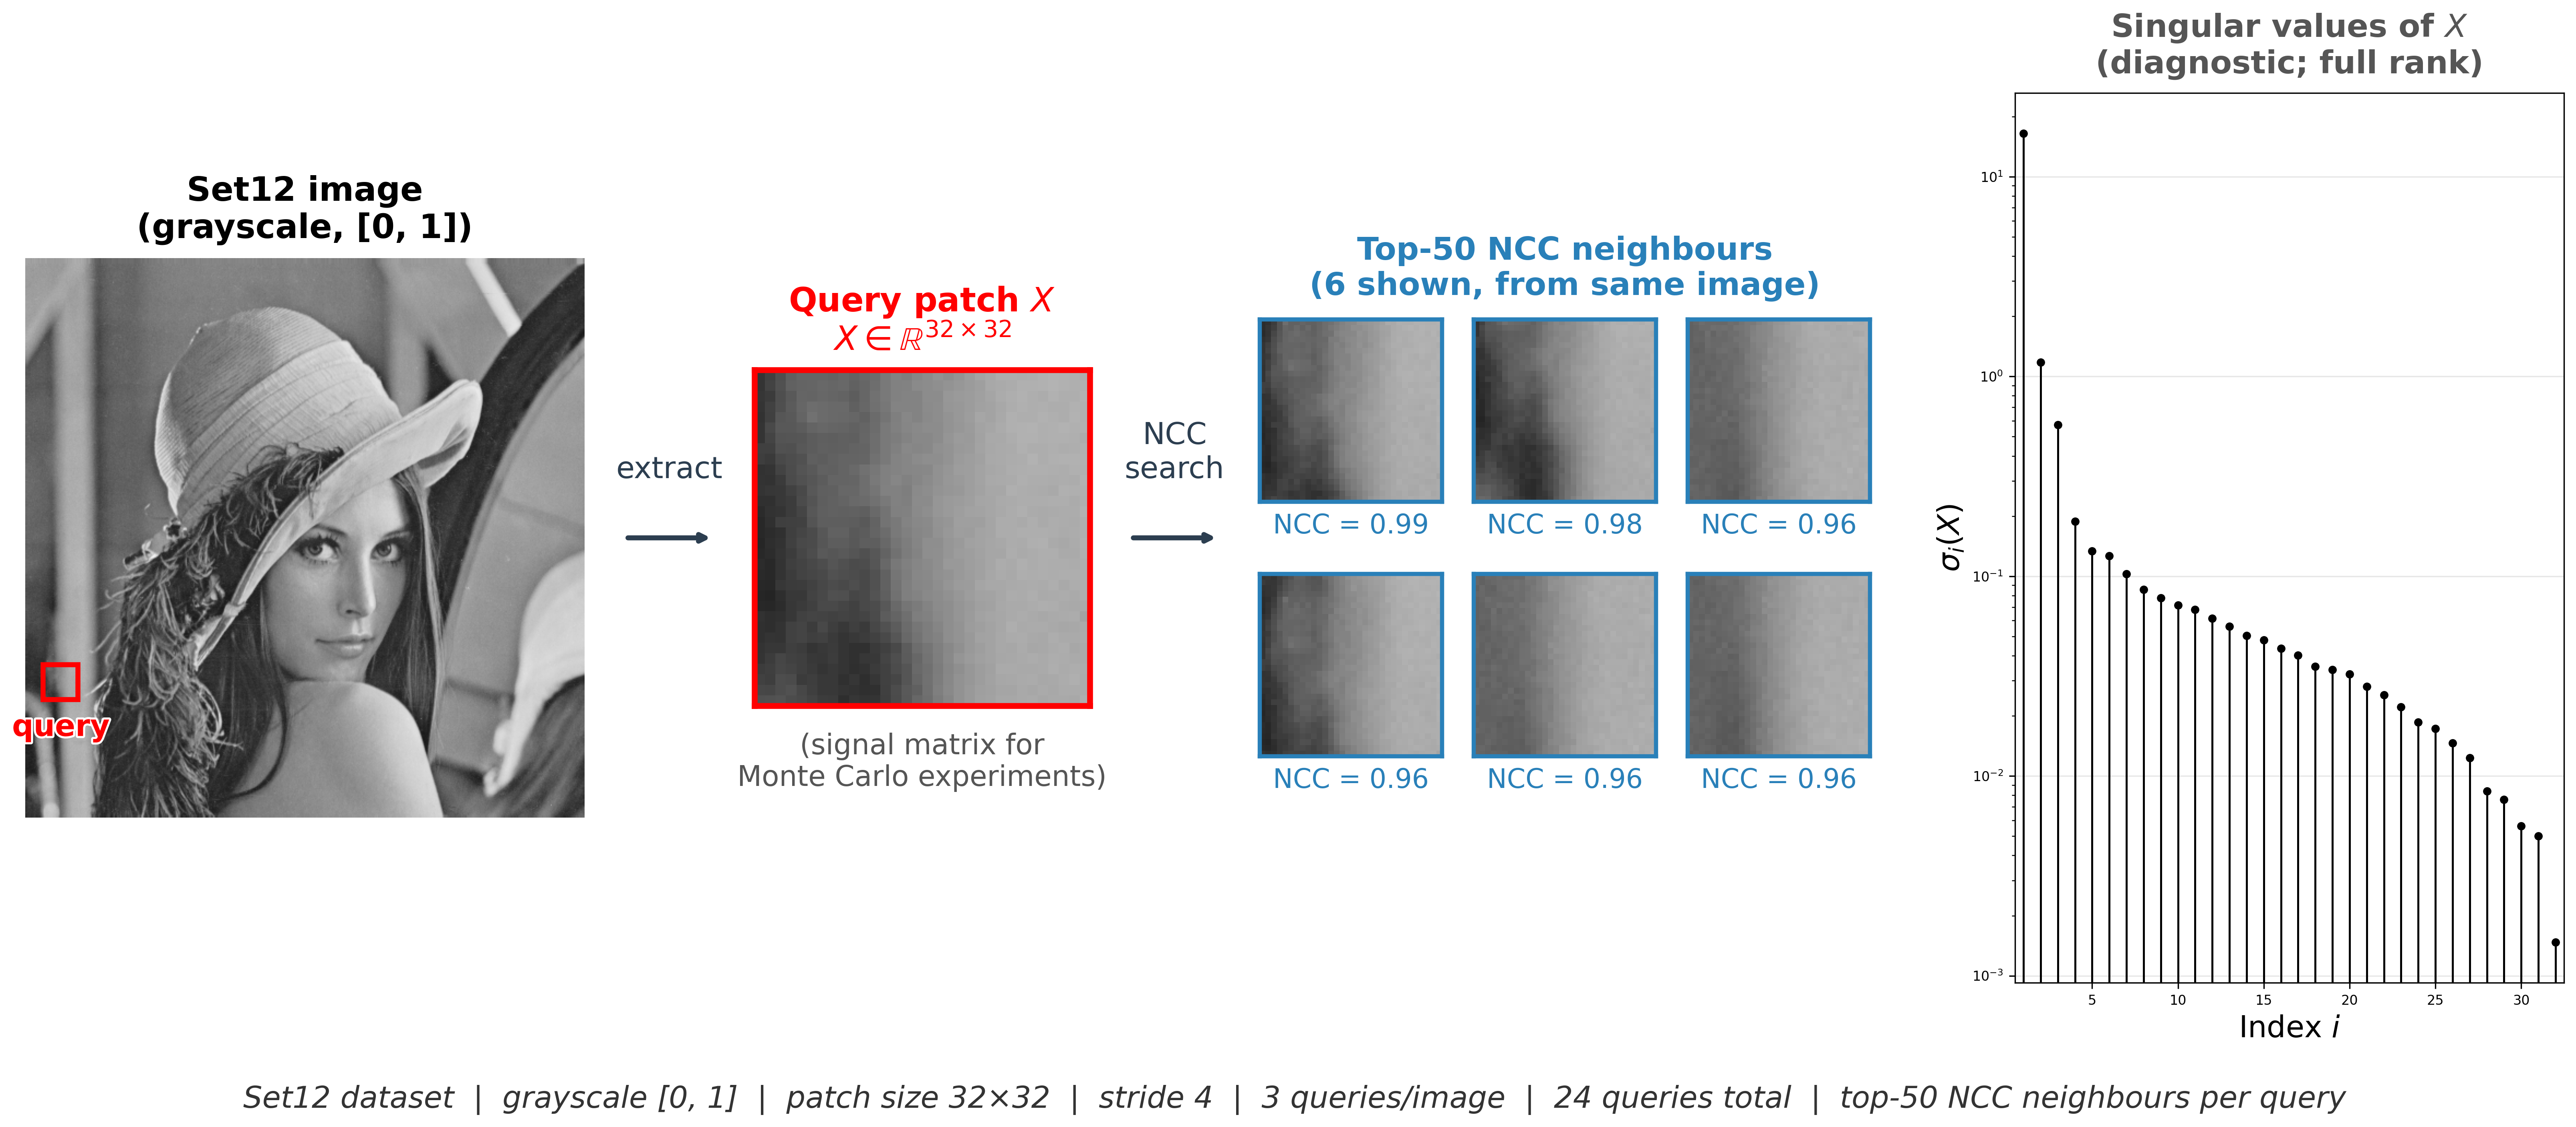
\includegraphics[width=1.28\textwidth]{figures/fig_diagnostic_patch_group_schematic.png}}
\par\smallskip
{\scriptsize Patch construction schematic: a query patch is extracted from a normalized grayscale image, compared with patches from the same image by normalized cross-correlation, and associated with its nearest patch neighbours. The matrix-level experiments below use the query patch itself as the clean matrix $X$.\par}
\end{center}

\subsection{Monte Carlo check of fixed-threshold unbiasedness}

The first experiment tests Proposition \ref{prop:sure-unbiased} with fixed deterministic $(\omega,\lambda)$. Over independent replicates we compare
\begin{equation}
    \widehat R_{\omega,
    \lambda}
    =\frac{1}{N}\sum_{r=1}^{N}
    \norm{\widehat X_{\omega,
    \lambda}(Y_r)-X}_F^2,
    \qquad
    \widehat S_{\omega,
    \lambda}
    =\frac{1}{N}\sum_{r=1}^{N}
    \operatorname{SURE}_{\omega,
    \lambda}(Y_r)
\end{equation}
which should agree up to Monte Carlo error.

Figure \ref{fig:exp1-sure-unbiasedness} shows the expected agreement. Panel (a) compares Monte Carlo mean SURE with Monte Carlo mean loss, and panel (b) reports the absolute relative discrepancy
\begin{equation}
    \frac{|\widehat S_{\omega,
    \lambda}-\widehat R_{\omega,
    \lambda}|}{\widehat R_{\omega,
    \lambda}}
\end{equation}
as a function of $\omega$. The discrepancies remain small over the tested range of smoothing parameters, including large $\omega$ where the logistic shrinker
is close to hard thresholding away from the threshold. This is consistent with the theoretical statement. The observed nonzero discrepancies are finite Monte Carlo errors, not evidence of systematic bias.

\begin{figure}[t]
\centering
\begin{minipage}[t]{0.47\textwidth}
\centering
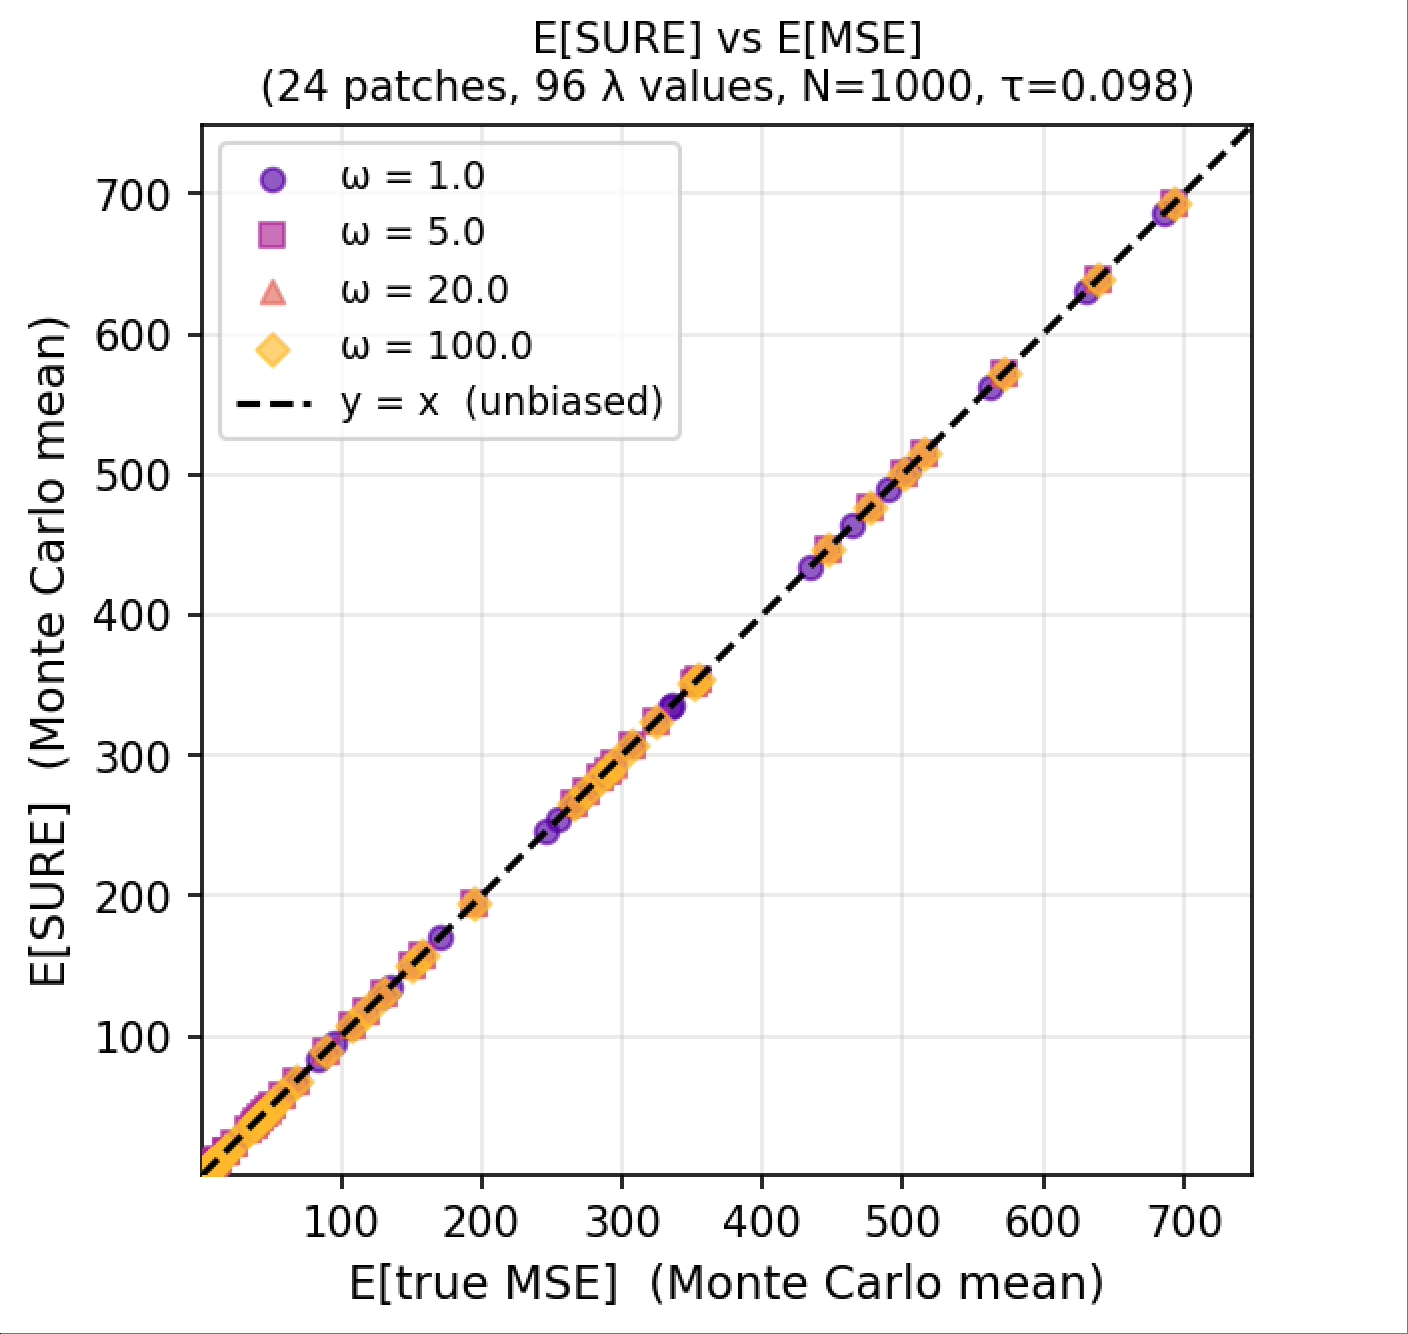
\includegraphics[width=\textwidth]{figures/exp1_sure_scatter.png}
\par\smallskip
{\small (a) Monte Carlo mean SURE versus Monte Carlo mean true loss for fixed $(\lambda,\omega)$.}
\end{minipage}\hfill
\begin{minipage}[t]{0.47\textwidth}
\centering
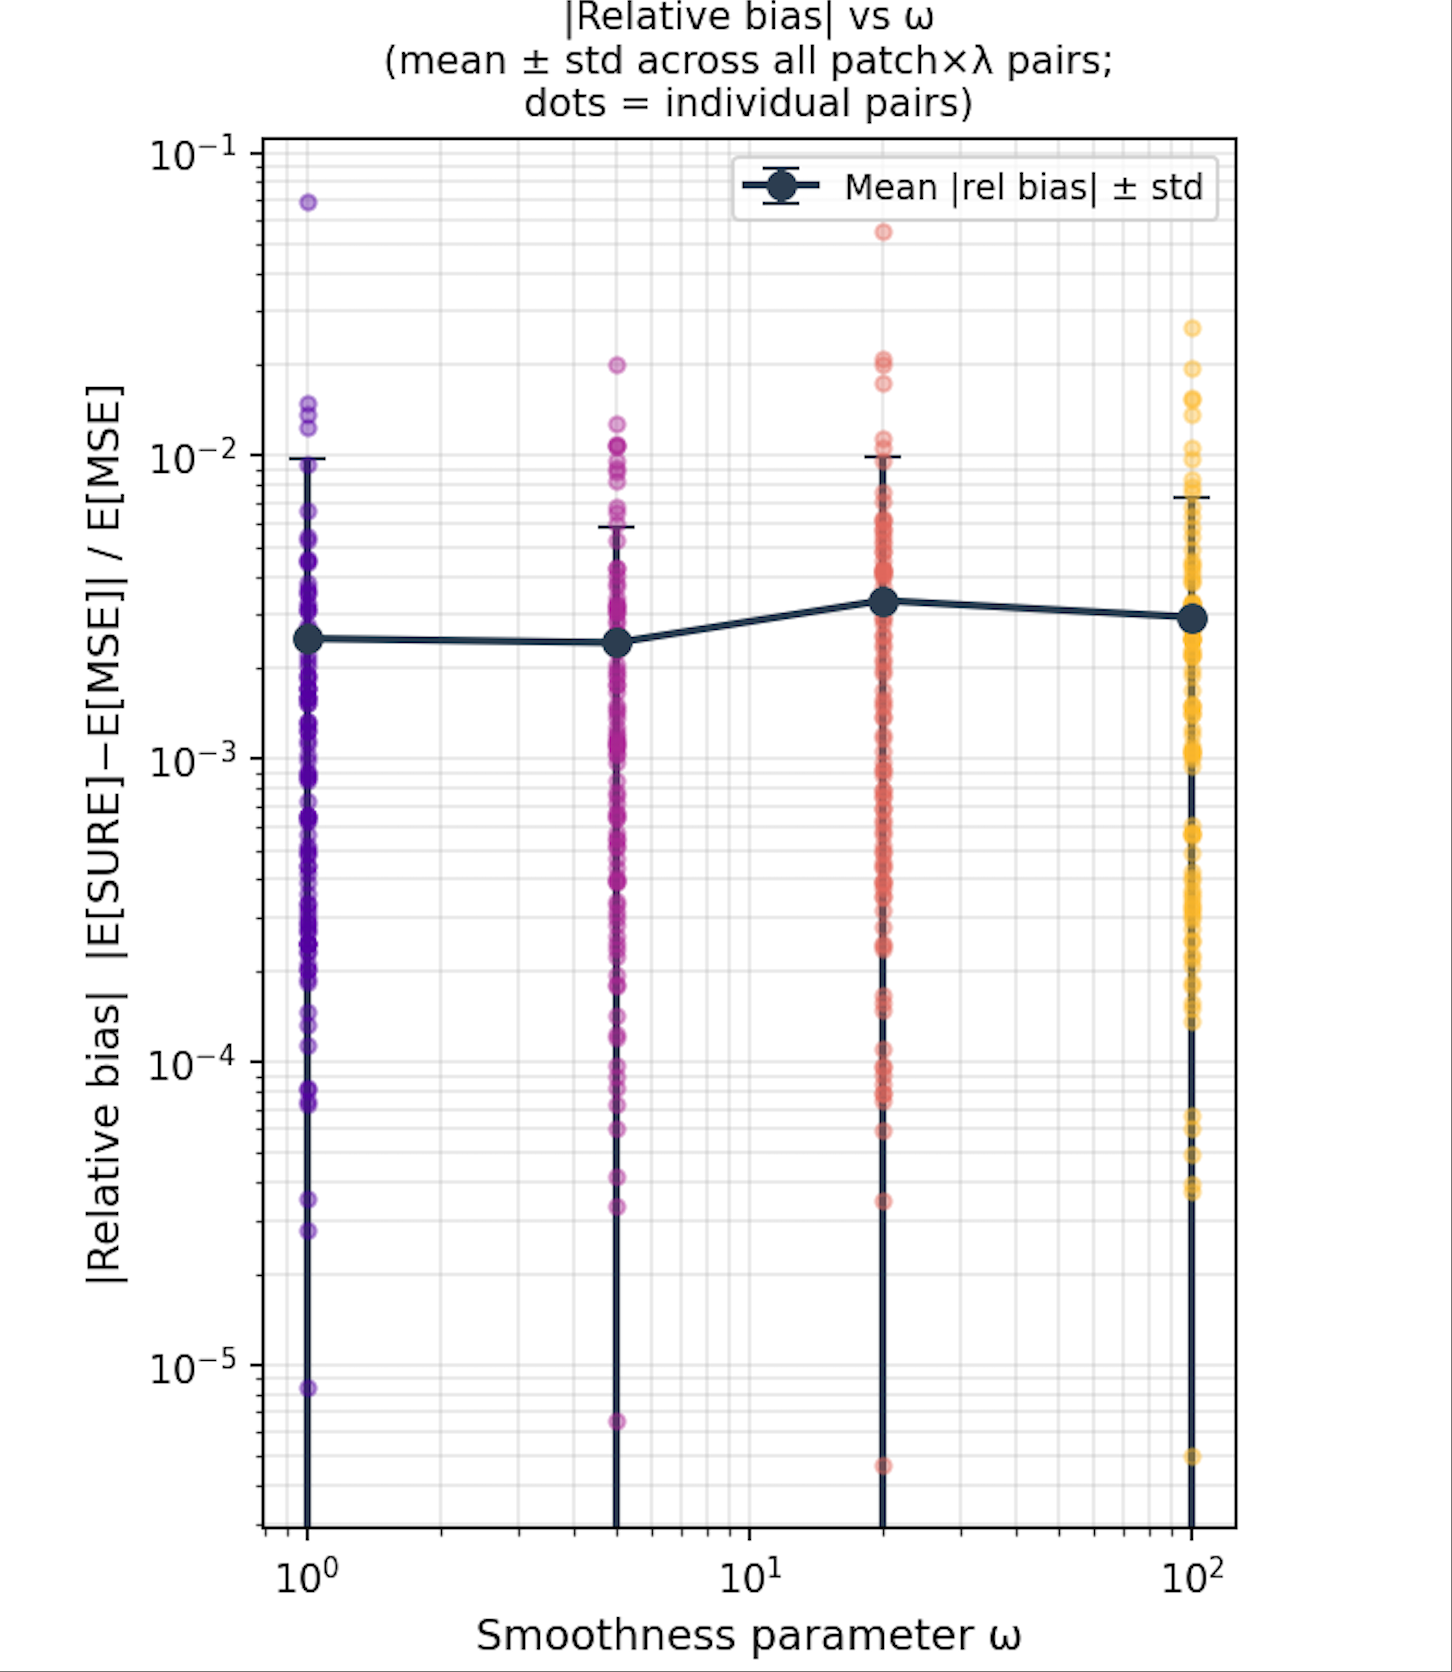
\includegraphics[width=\textwidth]{figures/exp1_relative_bias.png}
\par\smallskip
{\small (b) Absolute relative discrepancy as a function of the smoothness parameter $\omega$.}
\end{minipage}
\caption{Monte Carlo verification of the fixed-threshold identity in Proposition \ref{prop:sure-unbiased}. The thresholds are deterministic in this experiment, so the setup matches the hypotheses of the SURE theorem. The agreement between the Monte Carlo mean SURE and the Monte Carlo mean true loss confirms the implementation of \eqref{eq:smooth-sure} up to simulation error.}
\label{fig:exp1-sure-unbiasedness}
\end{figure}

\subsection{Post-selection optimism and low-risk rank selection}

The second experiment illustrates the caveat in Section 4. For each noisy matrix, the limiting scores are minimized over a finite rank set $\mathcal H$ to select rank:
\begin{equation}
    \widehat h_{\mathrm{SURE}}(Y_r)
    \in\arg\min_{h\in\mathcal H} S_h(Y_r).
\end{equation}
The selected score $S_{\widehat h_{\mathrm{SURE}}}(Y_r)$ is compared with the true loss of the selected estimator and with the oracle rank
\begin{equation}
    h_{\mathrm{or}}(Y_r)
    \in\arg\min_{h\in\mathcal H} L(\widehat X_h;X,Y_r),
\end{equation}
where $\widehat X_h$ is the hard rank-$h$ truncation. This oracle is used only to measure how much excess loss is incurred by the data-driven rank selection.

Figure \ref{fig:exp2-postselection} shows both effects: the selected SURE score is optimistic as a risk estimate, but the SURE-selected rank has true loss close to the oracle. Thus the score is used as a tuning criterion, not as an unbiased post-selection risk estimate.

\begin{figure}[t]
\centering
\begin{minipage}[t]{0.43\textwidth}
\centering
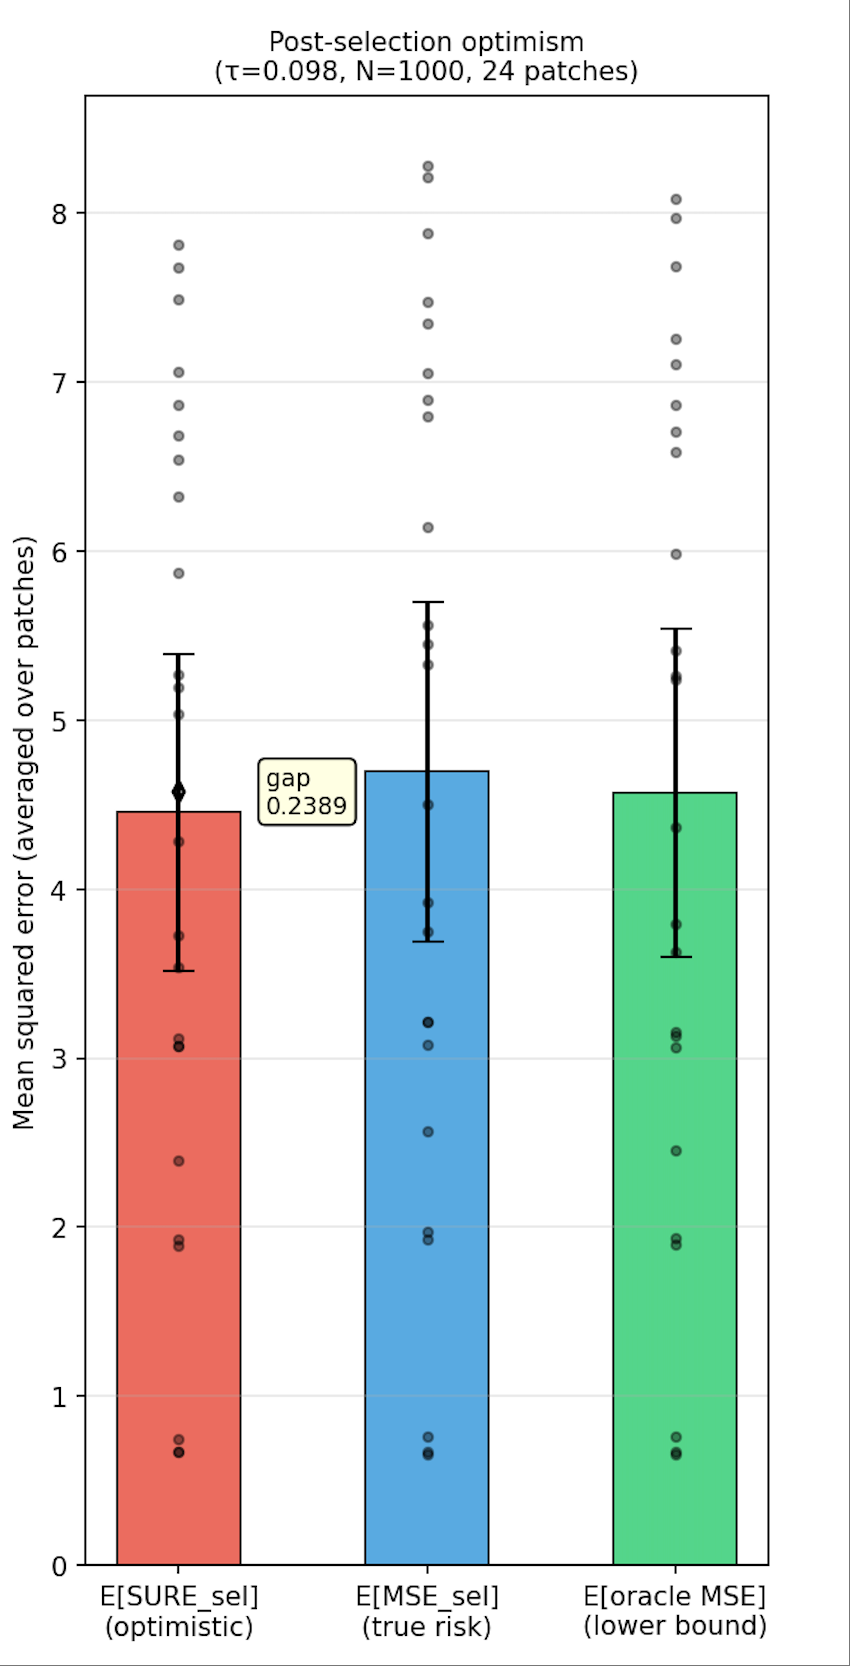
\includegraphics[width=\textwidth]{figures/exp2_postselection_bar.png}
\par\smallskip
{\small (a) Selected SURE score, selected true loss, and oracle loss.}
\end{minipage}\hfill
\begin{minipage}[t]{0.47\textwidth}
\centering
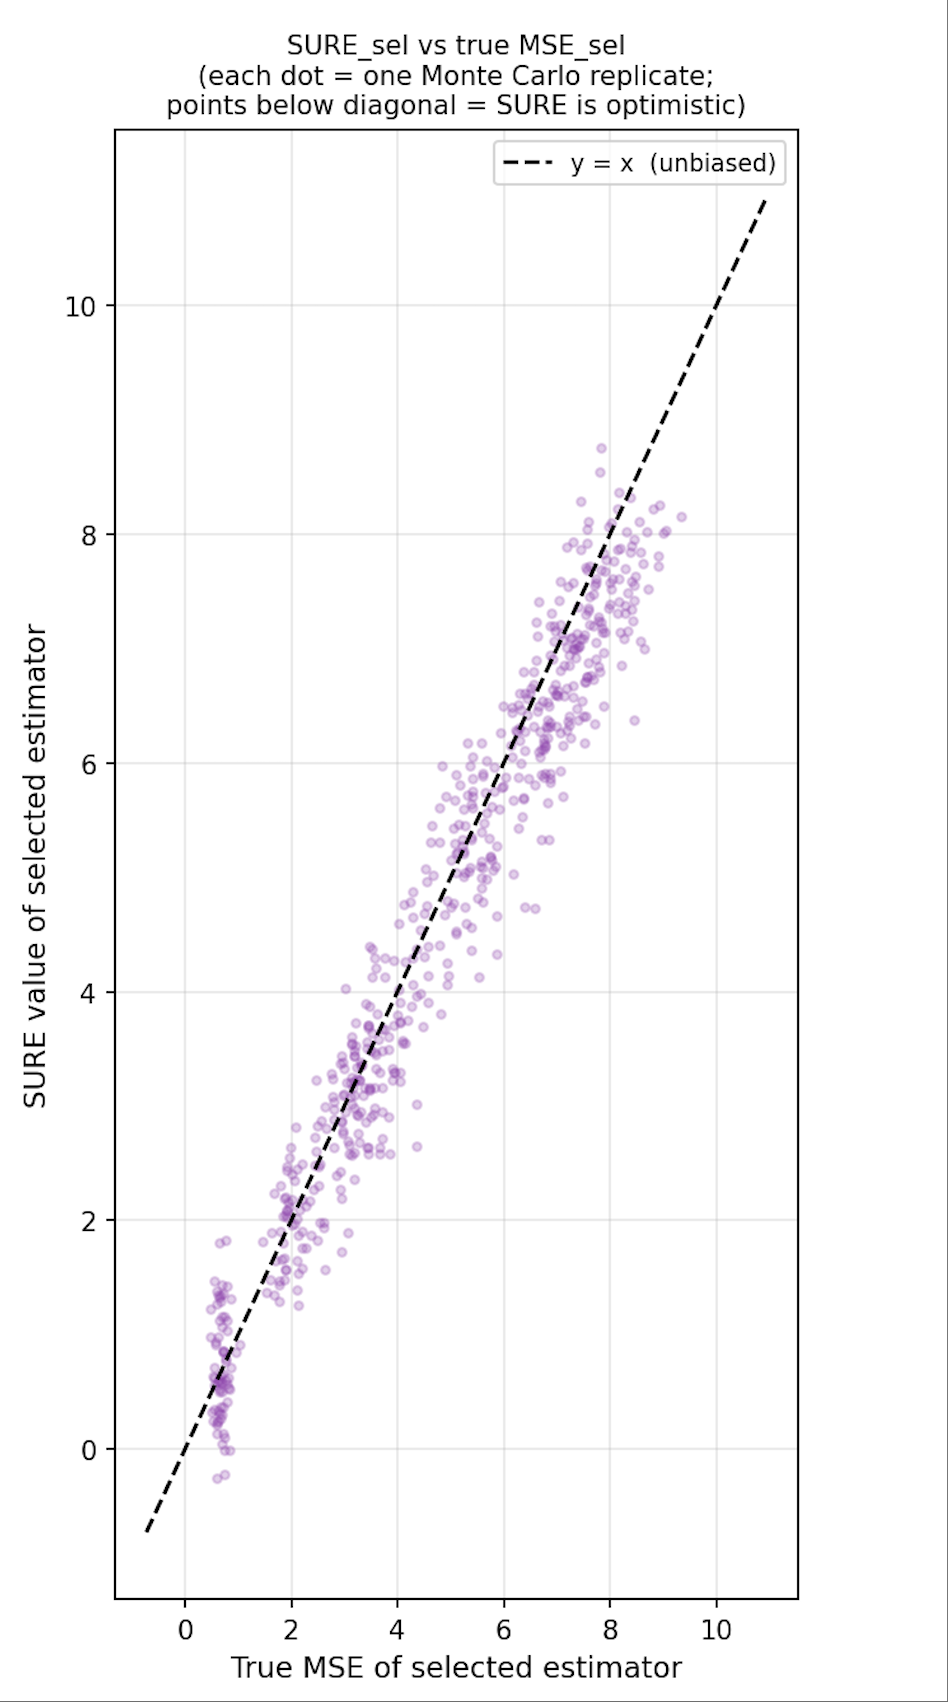
\includegraphics[width=\textwidth]{figures/exp2_postselection_scatter.png}
\par\smallskip
{\small (b) Replicate-level selected SURE score versus selected true loss.}
\end{minipage}
\caption{Post-selection behaviour of the plug-in ranking step. The selected SURE value is optimistic after minimization over candidate ranks, as shown by the gap between selected SURE and selected true loss and by the scatter plot lying below the diagonal. At the same time, the true loss of the SURE-selected rank is close to the oracle loss, showing that the ranking rule can still choose a low-risk rank.}
\label{fig:exp2-postselection}
\end{figure}

\subsection{Oracle-style comparison with energy matching}

The third experiment compares oracle, SURE and residual-energy rank selection over several noise levels $\tau$. The oracle rule chooses the best rank using $X$ and is included only as a benchmark.

For a method $M$, define its empirical oracle efficiency at noise level $\tau$ by
\begin{equation}
    \operatorname{Eff}_{\tau}(M)
    =\frac{\widehat{\E}_{\tau}\,L(\widehat X_{h_{\mathrm{or}}};X,Y)}
    {\widehat{\E}_{\tau}\,L(\widehat X_{h_M};X,Y)}.
\end{equation}
Values close to one indicate near-oracle performance, while smaller values indicate larger excess risk.

Figure \ref{fig:exp3-oracle-comparison} shows that SURE closely tracks the oracle curve and has higher oracle efficiency than residual-energy matching, consistent with the degrees-of-freedom correction in the SURE score.

\begin{figure}[t]
\centering
\begin{minipage}[t]{0.48\textwidth}
\centering
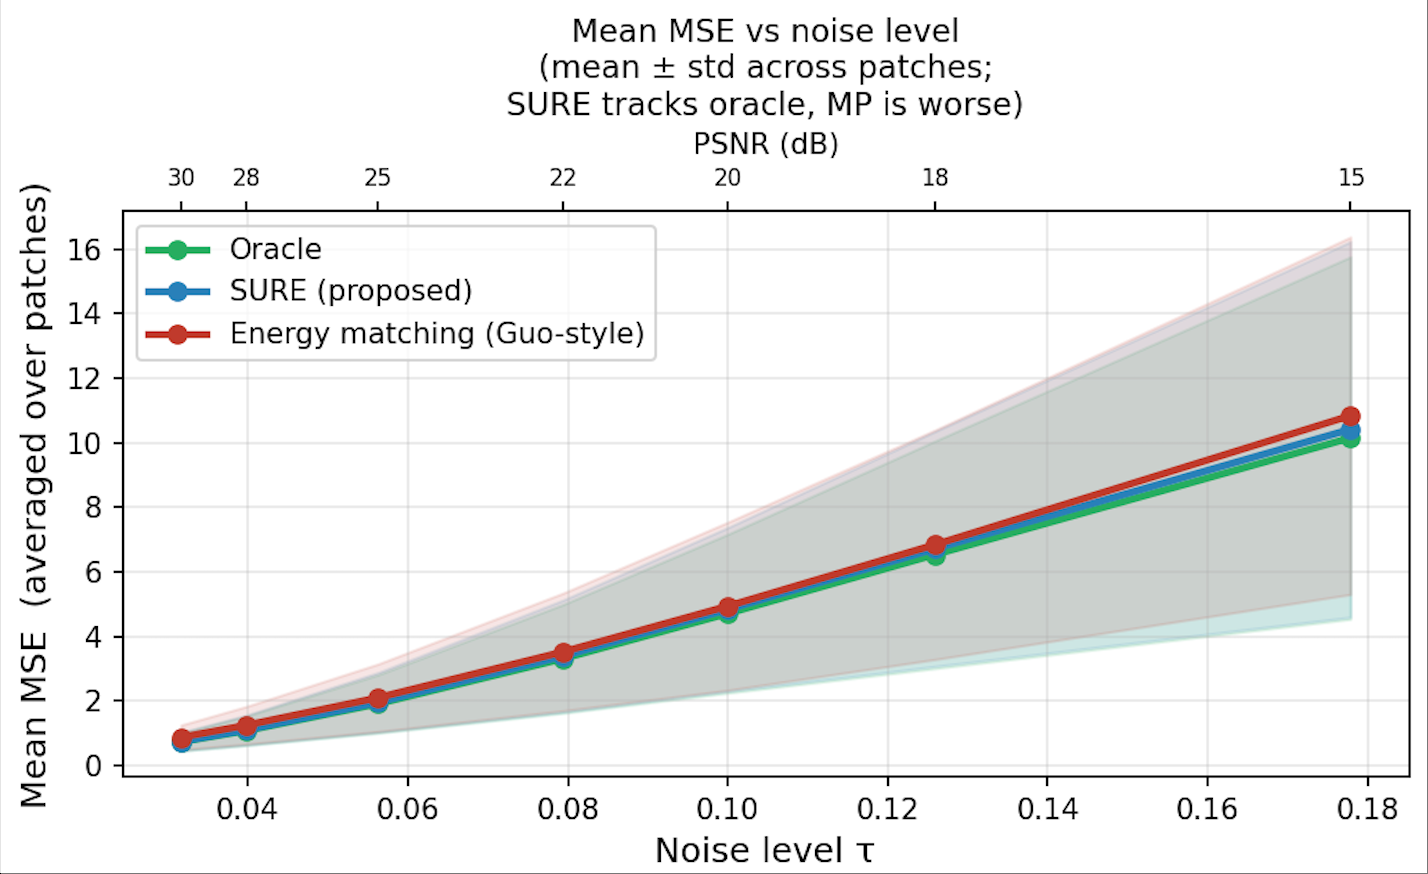
\includegraphics[width=\textwidth]{figures/exp3_mse_vs_tau.png}
\par\smallskip
{\small (a) Mean MSE as a function of the noise standard deviation $\tau$.}
\end{minipage}\hfill
\begin{minipage}[t]{0.48\textwidth}
\centering
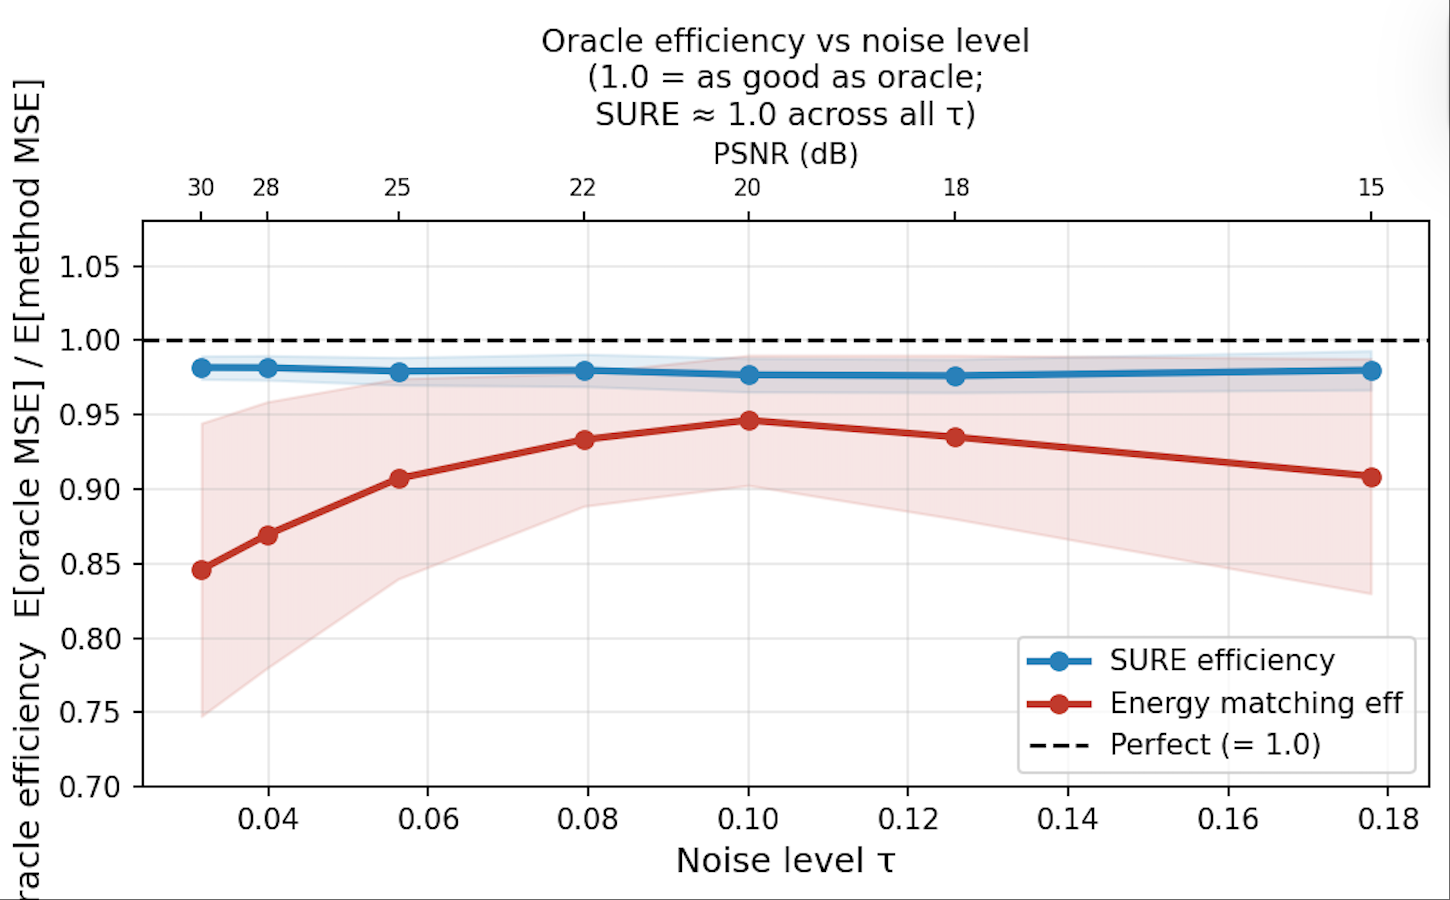
\includegraphics[width=\textwidth]{figures/exp3_efficiency_vs_tau.png}
\par\smallskip
{\small (b) Oracle efficiency as a function of $\tau$.}
\end{minipage}
\caption{Oracle-style comparison of rank-selection rules. The proposed SURE rule remains close to the oracle benchmark across the tested noise levels, while the residual-energy matching baseline has larger excess risk and lower oracle efficiency. The oracle is not implementable in practice; it is used only to quantify the excess loss of the data-driven rules.}
\label{fig:exp3-oracle-comparison}
\end{figure}


\subsection{Complete SVD denoising pipelines}

The preceding experiments isolate rank selection for one noisy matrix. The image-denoising experiment applies the same local SVD truncation primitive to patch-group matrices. In the synthetic setting one observes
\begin{equation}
    Y=X+W,
    \qquad W_{ab}\stackrel{\mathrm{i.i.d.}}{\sim}N(0,\tau^2),
\end{equation}
computes the SVD of $Y$, selects a rank $h$, and returns the hard rank-$h$ truncation. In the image setting this operation is applied to group matrices $P_j\in\R^{m\times n_j}$ formed from similar patches. This is an algorithmic transfer, not a direct application of the fixed deterministic-matrix model, because grouping, overlap, aggregation and back projection are data-dependent pipeline operations.

The original method of Guo et al.\ \cite{guo2016efficient} uses residual-energy matching: for $P_j\in\R^{m\times n_j}$ with $k_j=\min(m,n_j)$ and singular values $\sigma_{j,1}\geq\cdots\geq\sigma_{j,k_j}$, it chooses the smallest rank satisfying
\begin{equation}
    \sum_{i=h+1}^{k_j}\sigma_{j,i}^{2}
    \leq m n_j\tau^2.
\end{equation}
The SURE-modified method keeps the pipeline fixed but replaces this local rank rule by
\begin{equation}
\begin{aligned}
    S_0(P_j)&=\norm{P_j}_F^2-m n_j\tau^2,\\[-0.2em]
    S_h(P_j)&=-m n_j\tau^2+
    \sum_{i=h+1}^{k_j}\sigma_{j,i}^{2}\\[-0.2em]
    &\quad+2\tau^2\Biggl\{|m-n_j|h+h\\[-0.2em]
    &\qquad\qquad
    +2\sum_{i=1}^{h}\sum_{\substack{\ell=1\\ \ell\neq i}}^{k_j}
        \frac{\sigma_{j,i}^{2}}{\sigma_{j,i}^{2}-\sigma_{j,\ell}^{2}}
    \Biggr\},\quad h=1,\ldots,k_j,
\end{aligned}
\end{equation}
and selects
\begin{equation}
    \widehat h_j\in\arg\min_{0\leq h\leq k_j}S_h(P_j).
\end{equation}
The denoised group is the rank-$\widehat h_j$ hard truncation, so the only algorithmic substitution from the original pipeline to the proposed pipeline is the replacement of residual-energy matching by SURE limiting-score minimization.

Figure \ref{fig:sure-modified-pipeline} and Algorithm \ref{alg:sure-svd} summarize the modified pipeline and its implementation-level steps.

\clearpage

\begin{figure}[H]
\centering
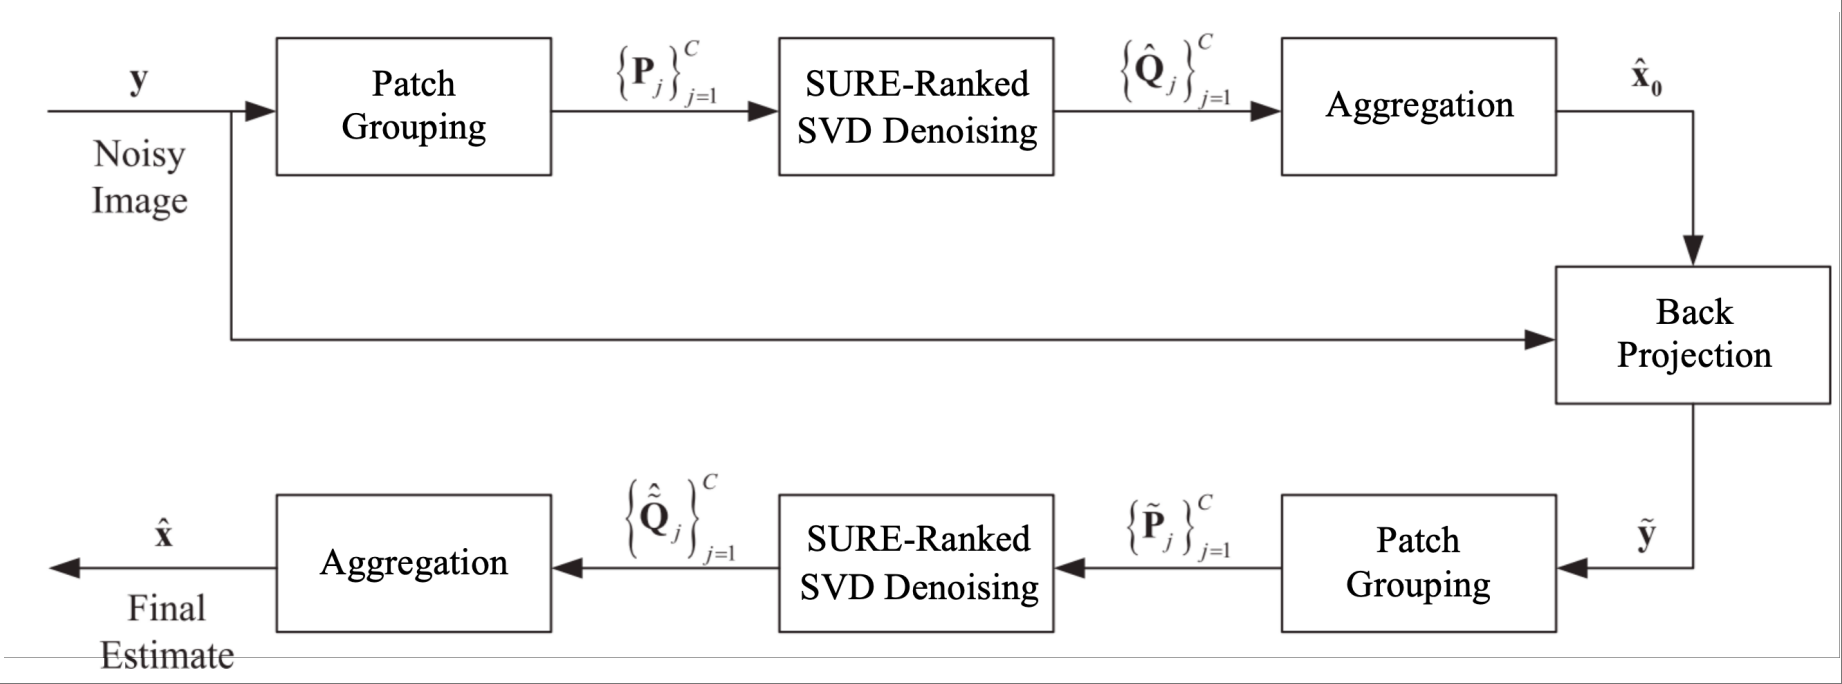
\includegraphics[width=0.80\textwidth]{figures/exp11.png}
\caption{SURE-modified two-pass SVD denoising pipeline. The method uses the original patch grouping, SVD truncation, aggregation, back projection, and refinement structure; only the local rank-selection rule inside each grouped-patch SVD block is changed.}
\label{fig:sure-modified-pipeline}
\end{figure}

\vspace{0.15em}
\begin{center}
\begin{minipage}{0.88\textwidth}
\refstepcounter{algorithm}\label{alg:sure-svd}
\hrule
\vspace{0.25em}
\noindent{\scriptsize\textbf{Algorithm \thealgorithm.} Proposed SURE-modified SVD denoising}
\vspace{0.25em}
\hrule
\vspace{0.25em}
{\tiny
\begin{algorithmic}[1]
\REQUIRE Noisy image $\mathbf y$ on the 8-bit intensity scale, noise standard deviation $\tau$ on the same scale
\ENSURE Denoised image $\widehat{\mathbf x}$
\STATE \textbf{Stage 1: initial denoising.}
\STATE Extract overlapping $\sqrt m\times\sqrt m$ patches from $\mathbf y$. For each reference patch, find the $L$ most similar patches using $S(\mathbf y_j,\mathbf y_c)=\|\mathbf y_j-\mathbf y_c\|_2^2$, and form $P_j=[\mathbf y_j,\mathbf y_{c,1},\ldots,\mathbf y_{c,L}]\in\R^{m\times n_j}$, where $n_j=L+1$.
\FOR{each group matrix $P_j$, $j=1,\ldots,C$}
    \STATE Compute $P_j=U_j\diagop(\sigma_{j,1},\ldots,\sigma_{j,k_j})V_j^T$, where $k_j=\min(m,n_j)$.
    \STATE Choose the SURE rank $\widehat h_j\in\arg\min_{h\in\{0,1,\ldots,k_j\}}S_h(P_j)$, where
    \[
    \begin{aligned}
    S_0(P_j)&=\|P_j\|_F^2-m n_j\tau^2,\\[-0.2em]
    S_h(P_j)&=-m n_j\tau^2+\sum_{i=h+1}^{k_j}\sigma_{j,i}^2 \\
    &\quad +2\tau^2\left\{|m-n_j|h+h
    +2\sum_{i=1}^{h}\sum_{\substack{\ell=1\\ \ell\neq i}}^{k_j}
    \frac{\sigma_{j,i}^2}{\sigma_{j,i}^2-\sigma_{j,\ell}^2}\right\},\quad h\geq1.
    \end{aligned}
    \]
    \STATE Set $\widehat Q_j=U_j\diagop(\sigma_{j,1},\ldots,\sigma_{j,\widehat h_j},0,\ldots,0)V_j^T$.
    \STATE Set $w_j=1-\widehat h_j/(L+1)$ if $\widehat h_j<L+1$, and $w_j=1/(L+1)$ otherwise.
\ENDFOR
\STATE Aggregate all $\widehat Q_j$ by weighted averaging to obtain $\widehat{\mathbf x}_0$.
\STATE \textbf{Back projection:} form $\widetilde{\mathbf y}=\widehat{\mathbf x}_0+\delta(\mathbf y-\widehat{\mathbf x}_0)$ with $\delta=0.5$, and update $\widetilde\tau=\gamma\sqrt{\max\{\tau^2-\|\widetilde{\mathbf y}-\widehat{\mathbf x}_0\|_F^2/(HW),0\}}$ with $\gamma=0.65$.
\STATE \textbf{Stage 2: refinement.} Repeat Stage~1 on $\widetilde{\mathbf y}$ with noise level $\widetilde\tau$ to obtain $\widehat{\mathbf x}$.
\end{algorithmic}
\medskip
\noindent\textbf{Parameters:} patch size $9\times9$ if $\tau<20$, $10\times10$ if $20\leq\tau<40$, and $11\times11$ if $\tau\geq40$; these thresholds use the 8-bit scale; similar patches $L=85$; search-window half-size $35$; reference-patch stride $3$.

\vspace{0.2em}
{\setlength{\baselineskip}{0.82\baselineskip}\selectfont
\noindent\textbf{Remark:} The only modification relative to Guo et al.\ \cite{guo2016efficient} is the rank-selection rule: energy matching is replaced by SURE-based limiting-score minimization. Patch grouping, SVD factorisation, truncation, aggregation and back projection remain identical.\par}
}
\vspace{0.25em}
\hrule
\end{minipage}
\end{center}

\clearpage

\subsection{Illustrative comparison with classical denoising methods}

We finally give an illustrative fixed-realization comparison involving K-SVD \cite{elad2006image}, LPG-PCA \cite{zhang2010two}, BM3D \cite{dabov2007image}, the original energy-matching SVD pipeline, and the SURE-modified SVD pipeline on Set12. The tested 8-bit noise levels are
\begin{equation}
    \sigma\in\{10,20,30,50\}
\end{equation}
For image index $i$, the noisy image is generated after setting
\begin{equation}
    \operatorname{rng}(100i+\sigma),
    \qquad
    y=x+\sigma Z,
    \qquad Z_{ab}\stackrel{\mathrm{i.i.d.}}{\sim}N(0,1).
\end{equation}
For each image--noise pair, all methods use the same single noisy realization. K-SVD uses Ron Rubinstein's MATLAB implementation (\texttt{ksvdbox13}, \texttt{ompbox10}) with parameters
\begin{equation}
\begin{gathered}
    \texttt{blocksize}=8,
    \quad \texttt{dictsize}=256,
    \quad \texttt{sigma}=\sigma,
    \quad \texttt{maxval}=255, \\
    \texttt{trainnum}=40000,
    \quad \texttt{iternum}=10,
    \quad \texttt{memusage}=\texttt{'high'}.
\end{gathered}
\end{equation}
LPG-PCA uses the official MATLAB code of Zhang et al. with profile \texttt{'fast'} and $K=0$. BM3D uses the Tampere University Python package \texttt{bm3d} version 4.0.3, with images normalized to $[0,1]$ and rescaled after denoising. The energy-matching and SURE columns are the controlled comparison of interest: they use identical Python pipeline code and differ only in the rank-selection function. The other methods are included only to provide context for the fixed-realization image-denoising scale. Their shared parameters are patch size $9\times9$, $10\times10$, or $11\times11$ according to noise level; $L=85$ similar patches; search-window half-size $35$; reference-patch stride $3$; back-projection parameter $\delta=0.5$; and, in the experiments, noise-update scaling factor $\gamma=0.65$.

PSNR is computed on the full image on the 8-bit scale. SSIM uses an $11\times11$ Gaussian window with standard deviation $1.5$, constants
\begin{equation}
    C_1=(0.01\cdot255)^2,
    \qquad
    C_2=(0.03\cdot255)^2,
\end{equation}
and the spatial average of the SSIM map, with equivalent MATLAB and Python convolution implementations.

\begin{table}[p]
\centering
\caption{PSNR and SSIM comparison on Set12 under additive white Gaussian noise. Noise levels are reported on the 8-bit intensity scale. Boldface marks the best PSNR and the best SSIM separately in each image--noise row, with ties included.}
\label{tab:final-comparison}
{\tiny
\setlength{\tabcolsep}{1.8pt}
\renewcommand{\arraystretch}{0.86}
\resizebox{\textwidth}{!}{%
\begin{tabular}{@{}ll*{5}{cc}@{}}
\toprule
Image & $\sigma$ & \multicolumn{2}{c}{K-SVD} & \multicolumn{2}{c}{LPG-PCA} & \multicolumn{2}{c}{BM3D} & \multicolumn{2}{c}{Energy matching} & \multicolumn{2}{c}{SURE proposed} \\
\cmidrule(lr){3-4}\cmidrule(lr){5-6}\cmidrule(lr){7-8}\cmidrule(lr){9-10}\cmidrule(l){11-12}
 & & PSNR & SSIM & PSNR & SSIM & PSNR & SSIM & PSNR & SSIM & PSNR & SSIM \\
\midrule
Cameraman & 10 & 33.64 & 0.9292 & 33.66 & 0.9258 & \textbf{34.08} & 0.9305 & \textbf{34.08} & \textbf{0.9357} & 33.65 & 0.9345 \\
 & 20 & 29.98 & 0.8668 & 29.97 & 0.8560 & \textbf{30.46} & 0.8680 & 30.33 & \textbf{0.8747} & 29.86 & 0.8527 \\
 & 30 & 28.01 & 0.8242 & 27.94 & 0.7958 & \textbf{28.65} & \textbf{0.8327} & 28.26 & 0.8275 & 28.26 & 0.8237 \\
 & 50 & 25.53 & 0.7543 & 25.47 & 0.7009 & \textbf{26.30} & \textbf{0.7714} & 25.32 & 0.7017 & 25.76 & 0.7684 \\
\addlinespace[0.15ex]
House & 10 & 36.01 & 0.9116 & 36.28 & 0.9162 & \textbf{36.77} & \textbf{0.9222} & 36.57 & 0.9178 & 36.61 & 0.9190 \\
 & 20 & 33.18 & 0.8698 & 33.10 & 0.8593 & 33.82 & 0.8734 & 33.57 & 0.8747 & \textbf{33.83} & \textbf{0.8774} \\
 & 30 & 31.26 & 0.8403 & 31.17 & 0.8106 & \textbf{32.33} & 0.8528 & 31.81 & 0.8534 & 32.26 & \textbf{0.8584} \\
 & 50 & 28.05 & 0.7780 & 28.27 & 0.7151 & 29.58 & 0.8100 & 28.65 & 0.8058 & \textbf{29.59} & \textbf{0.8203} \\
\addlinespace[0.15ex]
Pepper & 10 & 34.19 & 0.9278 & 34.06 & 0.9219 & 34.63 & 0.9304 & 34.56 & 0.9314 & \textbf{34.64} & \textbf{0.9320} \\
 & 20 & 30.75 & 0.8829 & 30.58 & 0.8680 & \textbf{31.35} & 0.8900 & 30.99 & 0.8886 & 31.13 & \textbf{0.8914} \\
 & 30 & 28.67 & 0.8443 & 28.40 & 0.8139 & \textbf{29.28} & \textbf{0.8537} & 28.67 & 0.8481 & 28.94 & 0.8529 \\
 & 50 & 26.15 & 0.7851 & 25.72 & 0.7191 & \textbf{26.82} & 0.7957 & 25.79 & 0.7881 & 26.42 & \textbf{0.7992} \\
\addlinespace[0.15ex]
Fishstar & 10 & 33.00 & 0.9306 & 33.17 & 0.9284 & 33.28 & 0.9296 & \textbf{33.57} & \textbf{0.9340} & 33.11 & 0.9295 \\
 & 20 & 29.19 & 0.8648 & 29.36 & 0.8586 & \textbf{29.69} & 0.8672 & 29.57 & 0.8670 & 29.64 & \textbf{0.8689} \\
 & 30 & 27.23 & 0.8153 & 27.31 & 0.8034 & \textbf{27.80} & 0.8246 & 27.53 & 0.8224 & 27.68 & \textbf{0.8274} \\
 & 50 & 24.28 & 0.7195 & 24.41 & 0.6954 & \textbf{25.06} & \textbf{0.7439} & 24.32 & 0.7225 & 24.53 & 0.7303 \\
\addlinespace[0.15ex]
Monarch & 10 & 33.75 & 0.9527 & 33.99 & 0.9526 & 34.20 & 0.9556 & \textbf{34.59} & \textbf{0.9612} & 34.31 & 0.9598 \\
 & 20 & 29.94 & 0.9128 & 29.98 & 0.9033 & 30.42 & 0.9184 & \textbf{30.53} & 0.9242 & \textbf{30.53} & \textbf{0.9257} \\
 & 30 & 27.80 & 0.8759 & 27.76 & 0.8582 & \textbf{28.42} & 0.8868 & 28.08 & 0.8828 & 28.35 & \textbf{0.8929} \\
 & 50 & 25.17 & 0.8051 & 24.96 & 0.7610 & \textbf{25.89} & 0.8220 & 25.14 & 0.8090 & 25.58 & \textbf{0.8225} \\
\addlinespace[0.15ex]
Airplane & 10 & 33.00 & 0.9249 & 33.00 & 0.9202 & \textbf{33.33} & \textbf{0.9288} & 33.26 & 0.9283 & 32.65 & 0.9255 \\
 & 20 & 29.34 & 0.8784 & 29.23 & 0.8609 & \textbf{29.65} & 0.8828 & 29.51 & \textbf{0.8844} & 29.52 & 0.8833 \\
 & 30 & 27.19 & 0.8336 & 27.10 & 0.7997 & \textbf{27.61} & \textbf{0.8431} & 27.38 & 0.8391 & 27.32 & 0.8378 \\
 & 50 & 24.56 & 0.7606 & 24.55 & 0.6900 & \textbf{25.33} & \textbf{0.7835} & 24.62 & 0.7674 & 24.73 & 0.7682 \\
\addlinespace[0.15ex]
Parrot & 10 & 33.18 & 0.9281 & 33.42 & 0.9261 & 33.53 & 0.9313 & \textbf{33.65} & \textbf{0.9336} & 33.10 & 0.9292 \\
 & 20 & 29.41 & 0.8661 & 29.61 & 0.8554 & 29.85 & 0.8720 & \textbf{29.90} & \textbf{0.8722} & 29.66 & 0.8690 \\
 & 30 & 27.54 & 0.8259 & 27.68 & 0.8020 & \textbf{28.01} & \textbf{0.8351} & 27.97 & 0.8316 & 27.99 & 0.8324 \\
 & 50 & 25.40 & 0.7704 & 25.29 & 0.7095 & \textbf{25.99} & \textbf{0.7875} & 25.77 & 0.7783 & 25.82 & 0.7810 \\
\addlinespace[0.15ex]
Lena & 10 & 35.48 & 0.9133 & 35.75 & 0.9136 & 35.93 & 0.9171 & \textbf{36.04} & \textbf{0.9192} & 35.92 & 0.9175 \\
 & 20 & 32.35 & 0.8668 & 32.49 & 0.8606 & 33.00 & 0.8775 & 32.88 & 0.8769 & \textbf{33.04} & \textbf{0.8792} \\
 & 30 & 30.46 & 0.8306 & 30.53 & 0.8072 & \textbf{31.25} & \textbf{0.8468} & 31.02 & 0.8445 & 31.16 & 0.8467 \\
 & 50 & 27.81 & 0.7674 & 27.99 & 0.7144 & \textbf{28.92} & \textbf{0.7963} & 28.13 & 0.7835 & 28.51 & 0.7910 \\
\addlinespace[0.15ex]
Barbara & 10 & 34.39 & 0.9361 & 35.02 & 0.9404 & 34.84 & 0.9409 & \textbf{35.41} & \textbf{0.9446} & 35.29 & 0.9444 \\
 & 20 & 30.75 & 0.8820 & 31.45 & 0.8948 & 31.69 & 0.9048 & 31.92 & 0.9072 & \textbf{32.15} & \textbf{0.9124} \\
 & 30 & 28.56 & 0.8266 & 29.24 & 0.8411 & 29.74 & 0.8669 & 29.62 & 0.8619 & \textbf{29.98} & \textbf{0.8729} \\
 & 50 & 25.38 & 0.7170 & 26.41 & 0.7373 & \textbf{27.04} & \textbf{0.7850} & 26.36 & 0.7654 & 26.94 & 0.7827 \\
\addlinespace[0.15ex]
Ship & 10 & 33.64 & 0.8868 & 33.72 & 0.8880 & \textbf{33.93} & 0.8893 & \textbf{33.93} & \textbf{0.8896} & 33.74 & 0.8857 \\
 & 20 & 30.26 & 0.8057 & 30.26 & 0.8062 & \textbf{30.85} & \textbf{0.8256} & 30.32 & 0.8051 & 30.45 & 0.8100 \\
 & 30 & 28.34 & 0.7472 & 28.27 & 0.7393 & \textbf{29.01} & \textbf{0.7736} & 28.32 & 0.7474 & 28.46 & 0.7524 \\
 & 50 & 25.88 & 0.6656 & 25.87 & 0.6340 & \textbf{26.67} & \textbf{0.6956} & 25.71 & 0.6643 & 26.05 & 0.6744 \\
\addlinespace[0.15ex]
Man & 10 & 33.54 & 0.9018 & 33.71 & 0.9025 & \textbf{34.01} & \textbf{0.9089} & 33.96 & 0.9077 & 33.71 & 0.9058 \\
 & 20 & 30.04 & 0.8164 & 30.12 & 0.8139 & \textbf{30.59} & \textbf{0.8317} & 30.22 & 0.8177 & 30.10 & 0.8115 \\
 & 30 & 28.17 & 0.7525 & 28.18 & 0.7413 & \textbf{28.77} & \textbf{0.7754} & 28.16 & 0.7506 & 28.19 & 0.7506 \\
 & 50 & 26.02 & 0.6697 & 26.05 & 0.6356 & \textbf{26.87} & \textbf{0.7047} & 25.87 & 0.6695 & 26.21 & 0.6809 \\
\addlinespace[0.15ex]
Couple & 10 & 33.52 & 0.9004 & 33.62 & 0.9011 & \textbf{34.03} & \textbf{0.9080} & 33.93 & 0.9063 & 33.71 & 0.9013 \\
 & 20 & 29.95 & 0.8178 & 30.07 & 0.8223 & \textbf{30.75} & \textbf{0.8438} & 30.32 & 0.8277 & 30.46 & 0.8330 \\
 & 30 & 27.94 & 0.7509 & 28.08 & 0.7542 & \textbf{28.92} & \textbf{0.7929} & 28.18 & 0.7643 & 28.39 & 0.7726 \\
 & 50 & 25.31 & 0.6425 & 25.50 & 0.6343 & \textbf{26.44} & \textbf{0.7034} & 25.25 & 0.6504 & 25.58 & 0.6665 \\
\midrule
Average &  & 29.65 & 0.8328 & 29.74 & 0.8169 & \textbf{30.32} & \textbf{0.8486} & 29.99 & 0.8398 & 30.07 & 0.8438 \\
\bottomrule
\end{tabular}%
}
}
\end{table}

\clearpage

Table \ref{tab:final-comparison} reports this fixed-realization comparison. BM3D, K-SVD and LPG-PCA are included as external reference points, but the controlled comparison for this paper is between the two SVD columns, where every pipeline component is shared except the rank-selection rule. In this setting, replacing residual-energy rank selection by SURE changes the average from $29.99/0.8398$ to $30.07/0.8438$, with improvements over energy matching in $32$ of $48$ PSNR entries and $31$ of $48$ SSIM entries. Because these are single noisy realizations and the average gain is small, these numbers should be read as modest descriptive evidence for the rank-selection replacement, not as a claim of statistical significance or superiority over existing denoising methods. The gains are strongest at the larger tested noise levels and are not uniform at $\sigma=10$. Figure \ref{fig:visual-house-sigma50} gives one qualitative high-noise example on House at $\sigma=50$.

\begin{figure}[H]
\centering
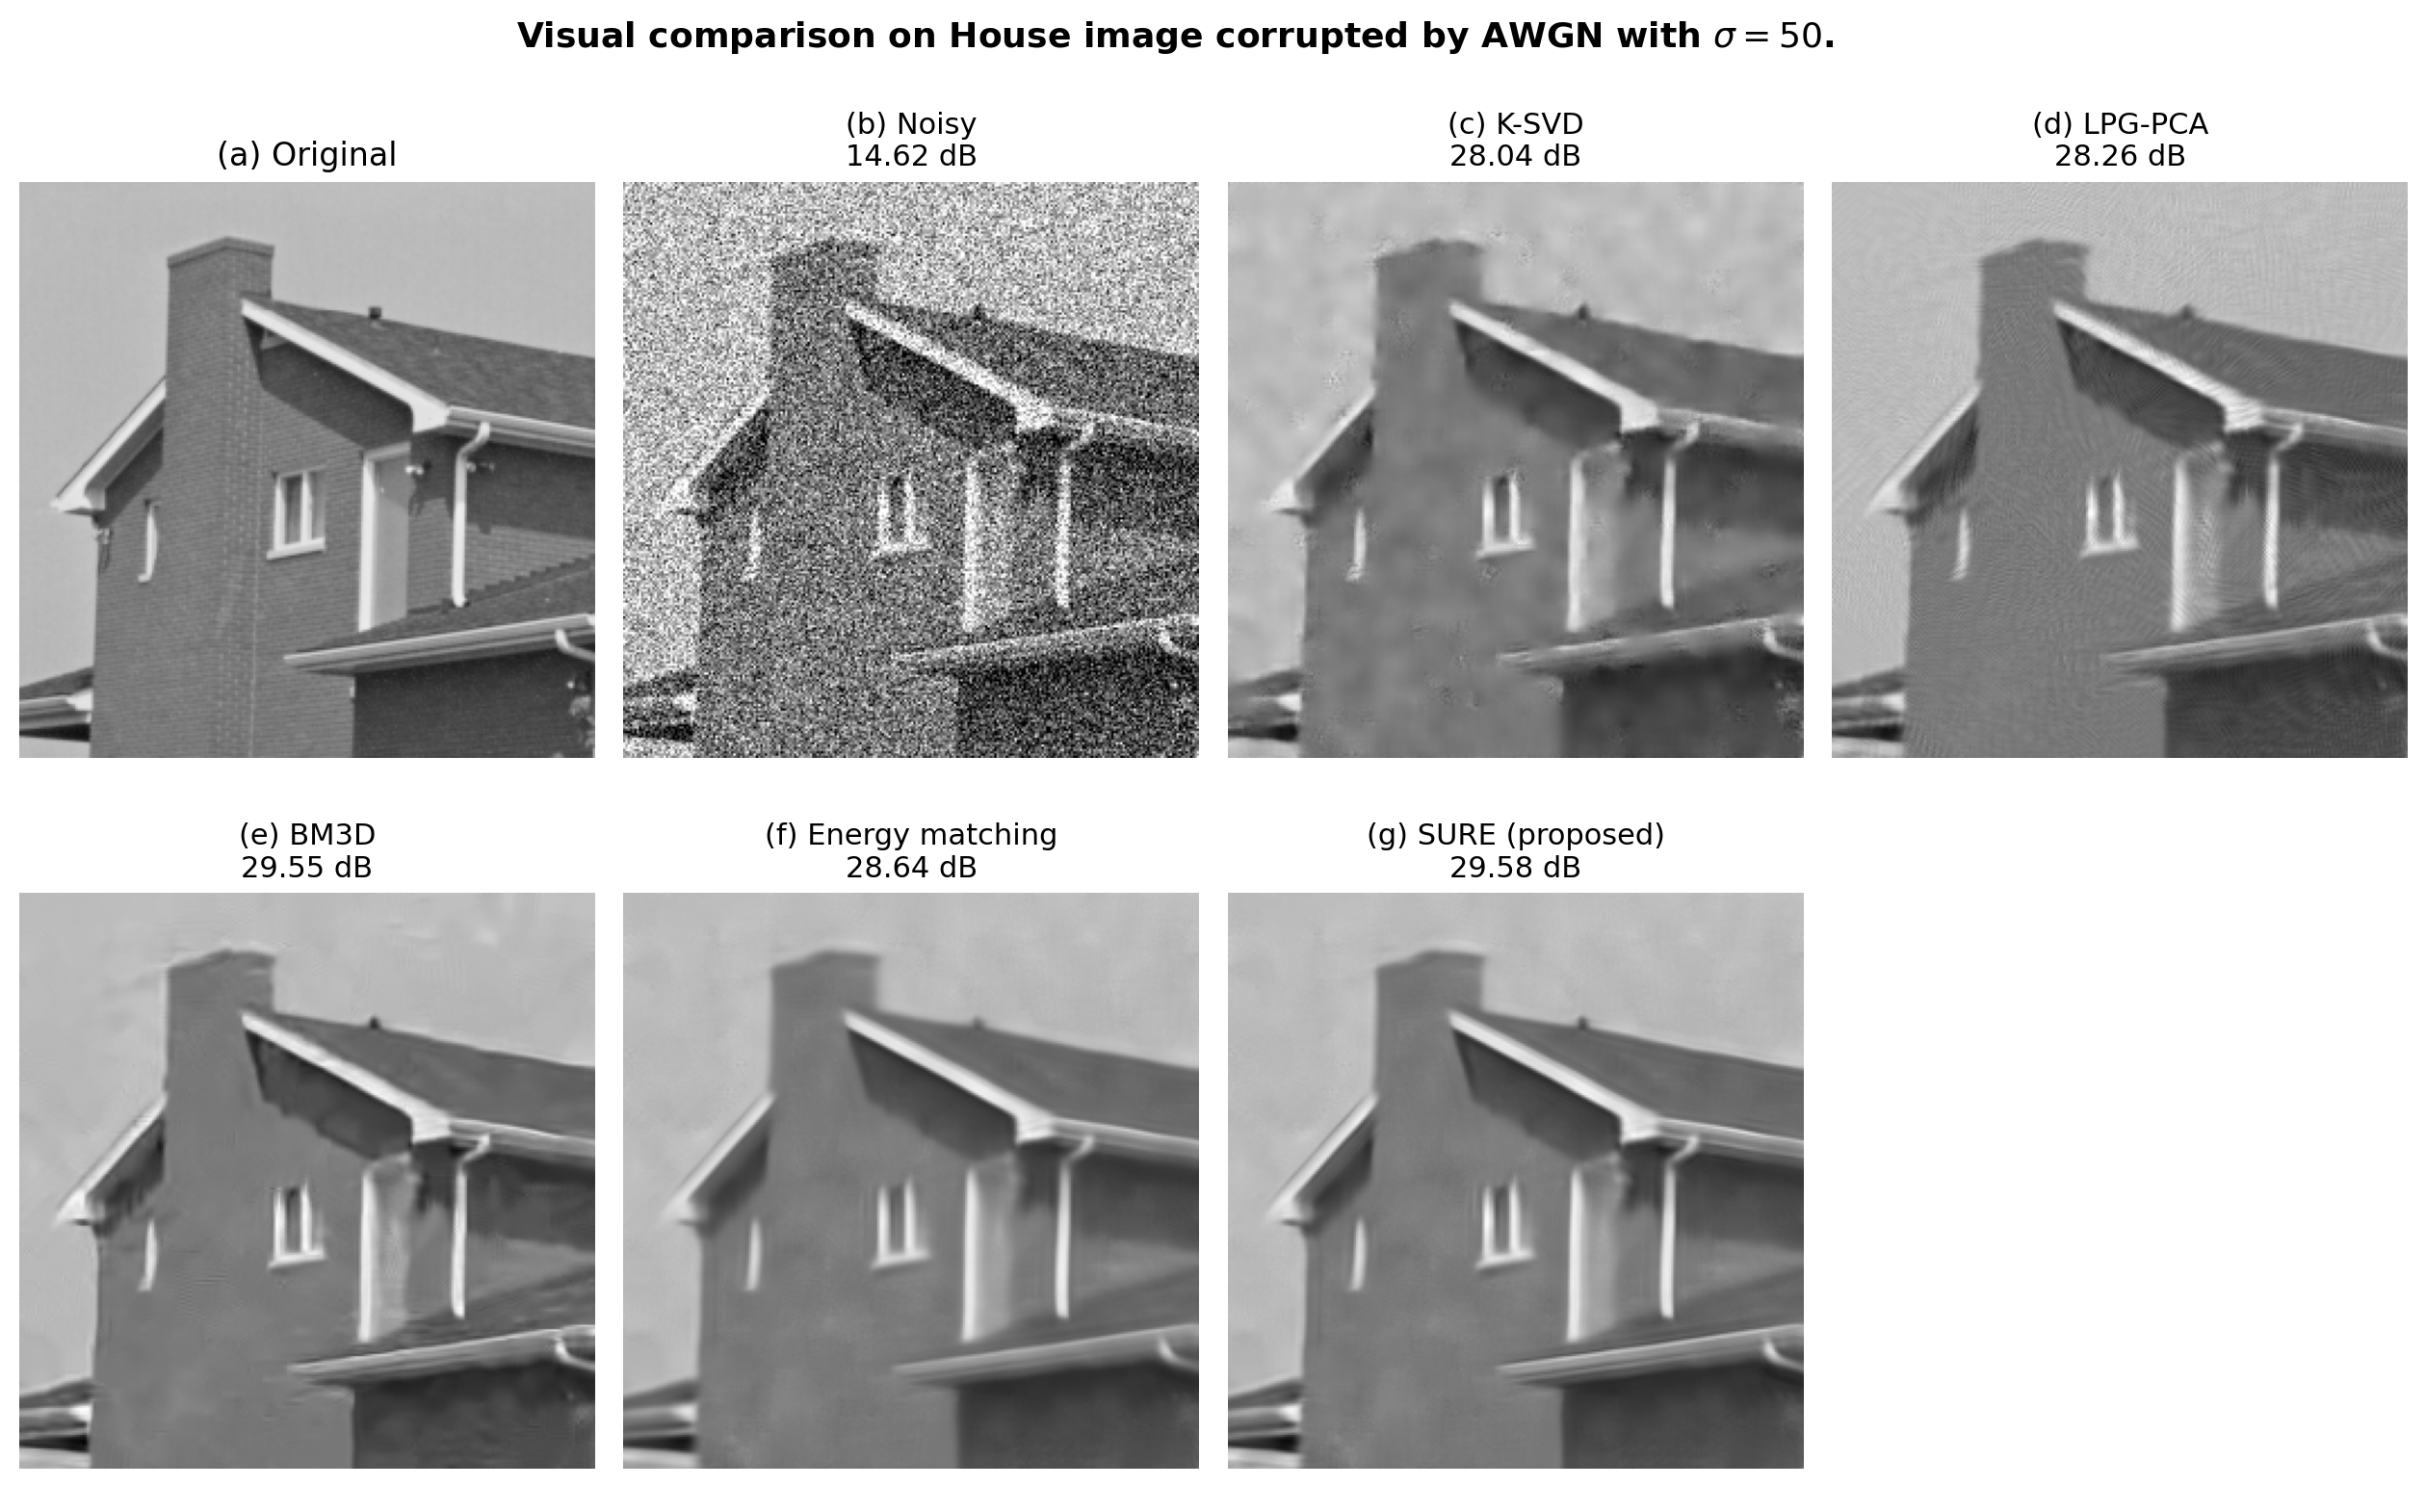
\includegraphics[width=0.88\textwidth]{figures/fig_visual_house_sigma50.png}
\caption{Illustrative visual comparison on the House image corrupted by additive white Gaussian noise with $\sigma=50$. Panels show the original image, the shared noisy input, and the denoised outputs from K-SVD, LPG-PCA, BM3D, energy matching, and the SURE-modified SVD pipeline. PSNR values are reported below the corresponding method labels for this single realization.}
\label{fig:visual-house-sigma50}
\end{figure}


\section{Conclusion and Discussion}

\paragraph{Contribution.}
This paper proposes a SURE-based threshold-ranking framework for SVD low-rank denoising. The central contribution is a reinterpretation of a biased hard-threshold SURE-like expression. We accept the negative result that singular value hard thresholding itself does not satisfy Stein's lemma \cite{hansen2017comment}; nevertheless, by introducing a smooth hard-threshold approximation, we obtain a fixed-threshold estimator whose SURE is exactly unbiased under Gaussian noise. For a fixed observed matrix and a finite candidate set separated from the singular values, strict inequalities in the limiting scores are eventually preserved by the smooth SURE objective as $\omega\to\infty$. This provides a computational ranking rule for finite-candidate SURE-based threshold tuning under the separation and post-selection caveats stated above. As in other data-driven SURE tuning methods, the selected threshold should be distinguished from the fixed-threshold estimators used to construct the unbiased risk estimates.

\paragraph{Limitations.}
The limitations are as follows. The ordering argument is finite-candidate and pointwise: thresholds must be separated from the observed singular values, and the result does not justify continuous optimization over all $\lambda\in\R$. The limiting score ranks candidates but is not an unbiased risk estimate for discontinuous hard thresholding or for a data-selected threshold. In the image pipeline, block matching and overlapping aggregation go beyond the fixed-matrix Gaussian model used in the proof. Finally, the denoising table is a fixed-realization comparison; multiple noisy seeds would be needed for standard errors or formal significance tests.

\paragraph{Future work.}
Future work includes broader matrix and image benchmarks, post-selection risk correction, extensions to other nonsmooth estimators, and a controlled continuous-threshold theory compatible with the fixed-threshold SURE interpretation.

\begin{thebibliography}{14}

\bibitem{stein1981estimation}
C. M. Stein.
\newblock Estimation of the mean of a multivariate normal distribution.
\newblock \emph{The Annals of Statistics}, 9(6):1135--1151, 1981.

\bibitem{andersson2016operator}
F. Andersson, M. Carlsson, and K.-M. Perfekt.
\newblock Operator-Lipschitz estimates for the singular value functional calculus.
\newblock \emph{Proceedings of the American Mathematical Society}, 144(5):1867--1875, 2016.

\bibitem{candes2013unbiased}
E. J. Cand\`es, C. A. Sing-Long, and J. D. Trzasko.
\newblock Unbiased risk estimates for singular value thresholding and spectral estimators.
\newblock \emph{IEEE Transactions on Signal Processing}, 61(19):4643--4657, 2013.

\bibitem{guo2016efficient}
Q. Guo, C. Zhang, Y. Zhang, and H. Liu.
\newblock An efficient SVD-based method for image denoising.
\newblock \emph{IEEE Transactions on Circuits and Systems for Video Technology}, 26(5):868--880, 2016.

\bibitem{elad2006image}
M. Elad and M. Aharon.
\newblock Image denoising via sparse and redundant representations over learned dictionaries.
\newblock \emph{IEEE Transactions on Image Processing}, 15(12):3736--3745, 2006.

\bibitem{zhang2010two}
L. Zhang, W. Dong, D. Zhang, and G. Shi.
\newblock Two-stage image denoising by principal component analysis with local pixel grouping.
\newblock \emph{Pattern Recognition}, 43(4):1531--1549, 2010.

\bibitem{dabov2007image}
K. Dabov, A. Foi, V. Katkovnik, and K. Egiazarian.
\newblock Image denoising by sparse 3-D transform-domain collaborative filtering.
\newblock \emph{IEEE Transactions on Image Processing}, 16(8):2080--2095, 2007.

\bibitem{mukherjee2015degrees}
A. Mukherjee, K. Chen, N. Wang, and J. Zhu.
\newblock On the degrees of freedom of reduced-rank estimators in multivariate regression.
\newblock \emph{Biometrika}, 102(2):457--477, 2015.

\bibitem{efron1986biased}
B. Efron.
\newblock How biased is the apparent error rate of a prediction rule?
\newblock \emph{Journal of the American Statistical Association}, 81(394):461--470, 1986.

\bibitem{efron2004prediction}
B. Efron.
\newblock The estimation of prediction error: covariance penalties and cross-validation.
\newblock \emph{Journal of the American Statistical Association}, 99(467):619--632, 2004.

\bibitem{hansen2017comment}
N. R. Hansen.
\newblock A comment on Stein's unbiased risk estimate for reduced rank estimators.
\newblock arXiv:1708.09657, 2017.

\end{thebibliography}

\end{document}
